\documentclass[main.tex,fontsize=8pt,paper=a4,paper=portrait,DIV=calc]{scrartcl}
% Document
\usepackage[T1]{fontenc}
\usepackage[dvipsnames]{xcolor}
\usepackage[nswissgerman,english]{babel}
\renewcommand{\familydefault}{\sfdefault}

% Format
\usepackage[top=5mm,bottom=1mm,left=5mm,right=5mm]{geometry}
%\setlength{\headheight}{\baselineskip}
%\setlength{\headsep}{0mm}

%\usepackage{scrlayer-scrpage}
%\clearpairofpagestyles
%\chead{{\bfseries\TITLE, \AUTHOR, \pagename~\thepage}}

%\addtokomafont{pagehead}{\upshape}

\usepackage{multicol}
\setlength{\columnsep}{2mm}
\setlength{\columnseprule}{0.1pt}

% Math
\usepackage{amsmath}
\usepackage{amssymb}
\usepackage{amsfonts}

% Code
\usepackage{fancyvrb, etoolbox, listings, xcolor}
%\usemintedstyle{bw}

%\newminted[shell]{bash}{
%fontsize=\footnotesize,
%fontfamily=tt,
%breaklines=true,
%frame=single,
%framerule=0.1pt,
%framesep=2mm,
%tabsize=2
%}
%\newminted{css}{
%breaklines=true,
%tabsize=4,
%autogobble=true,
%escapeinside=||,
%stripall=true,
%stripnl=true,
%}

    \definecolor{lightgray}{rgb}{0.95, 0.95, 0.95}
    \definecolor{darkgray}{rgb}{0.4, 0.4, 0.4}
    \definecolor{purple}{rgb}{0.65, 0.12, 0.82}
    \definecolor{ocherCode}{rgb}{1, 0.5, 0} % #FF7F00 -> rgb(239, 169, 0)
    \definecolor{blueCode}{rgb}{0, 0, 0.93} % #0000EE -> rgb(0, 0, 238)
    \definecolor{greenCode}{rgb}{0, 0.6, 0} % #009900 -> rgb(0, 153, 0)
    \definecolor{teal}{rgb}{0.0, 0.5, 0.5}

\lstdefinestyle{code}{
    identifierstyle=\color{black},
    keywordstyle=\color{blue}\bfseries\small,
    ndkeywordstyle=\color{greenCode}\bfseries\small,
    stringstyle=\color{ocherCode}\ttfamily\small,
    commentstyle=\color{teal}\ttfamily\textit\small,
    basicstyle=\ttfamily\small,
    breakatwhitespace=false,         
    breaklines=true,                 
    captionpos=b,                    
    keepspaces=true,                 
    showspaces=false,                
    showstringspaces=false,
    showtabs=false,                  
    tabsize=2,
    belowskip=-5pt
}



% Images
\usepackage{graphicx}
\newcommand{\pic}{\includegraphics[scale=0.3]}
\graphicspath{{Screenshots/}{../Screenshots}}
\makeatletter
\def\pictext#1#2{%
    \@ifnextchar[{%
    \pictext@iiiii{#1}{#2}%
    }{%
      \pictext@iiiii{#1}{#2}[0.5,0.4,0.3]% Default is 5
    }%
}
\def\pictext@iiiii#1#2[#3,#4,#5]{\begin{minipage}{#3\textwidth}\includegraphics[scale=#4]{#1}\end{minipage}\begin{minipage}{#5\textwidth}#2\end{minipage}}
\def\minipg#1#2{%
    \@ifnextchar[{%
    \minipg@iiii{#1}{#2}%
    }{%
      \minipg@iiii{#1}{#2}[0.3,0.6]% Default is 5
    }%
}
\def\minipg@iiii#1#2[#3,#4]{\vspace{0.8mm}\begin{minipage}{#3\textwidth}#1\end{minipage}\begin{minipage}{#4\textwidth}#2\end{minipage}{\vspace{0.8mm}}}
\makeatother

%\newenvironment{minty}[2]% environment name
%{% begin code
%  \begin{minipage}{#1}
%  \begin{minted}{#2}
%}%
%{% end code
%  \end{minted}
%  \end{minipage}
%  \end{minty}\ignorespacesafterend
%} 

% Smaller Lists
\usepackage{enumitem}
\setlist[itemize,enumerate]{leftmargin=3mm, labelindent=0mm, labelwidth=1mm, labelsep=1mm, nosep}
\setlist[description]{leftmargin=0mm, nosep}
\setlength{\parindent}{0cm}

% Smaller Titles
\usepackage[explicit]{titlesec}

%% Color Boxes
\newcommand{\sectioncolor}[1]{\colorbox{black!60}{\parbox{0.989\linewidth}{\color{white}#1}}}
\newcommand{\subsectioncolor}[1]{\colorbox{black!50}{\parbox{0.989\linewidth}{\color{white}#1}}}
\newcommand{\subsubsectioncolor}[1]{\colorbox{black!40}{\parbox{0.989\linewidth}{\color{white}#1}}}
\newcommand{\paragraphcolor}[1]{\colorbox{black!30}{\parbox{0.989\linewidth}{\color{white}#1}}}
\newcommand{\subparagraphcolor}[1]{\colorbox{black!20}{\parbox{0.989\linewidth}{\color{white}#1}}}

%% Title Format
\titleformat{\section}{\vspace{0.5mm}\bfseries}{}{0mm}{\sectioncolor{\thesection~#1}}[{\vspace{0.5mm}}]
\titleformat{\subsection}{\vspace{0.5mm}\bfseries}{}{0mm}{\subsectioncolor{\thesubsection~#1}}[{\vspace{0.5mm}}]
\titleformat{\subsubsection}{\vspace{0.5mm}\bfseries}{}{0mm}{\subsubsectioncolor{\thesubsubsection~#1}}[{\vspace{0.5mm}}]
\titleformat{\paragraph}{\vspace{0.5mm}\bfseries}{}{0mm}{\paragraphcolor{\theparagraph~#1}}[{\vspace{0.5mm}}]
\titleformat{\subparagraph}{\vspace{0.5mm}\bfseries}{}{0mm}{\subparagraphcolor{\thesubparagraph~#1}}[{\vspace{0.5mm}}]

%% Title Spacing
\titlespacing{\section}{0mm}{0mm}{0mm}
\titlespacing{\subsection}{0mm}{0mm}{0mm}
\titlespacing{\subsubsection}{0mm}{0mm}{0mm}
\titlespacing{\paragraph}{0mm}{0mm}{0mm}
\titlespacing{\subparagraph}{0mm}{0mm}{0mm}

%% format cells
\usepackage[document]{ragged2e}
\usepackage{array, makecell}
\renewcommand{\arraystretch}{2}
\newcommand{\mc}{\makecell[{{m{1\linewidth}}}]}



\lstset{
    language=c++,
    style=code,
}
%%%%%

\title{C++}
\author{Fabio Lenherr}

\pagestyle{plain}
\pagenumbering{arabic}
\begin{document}
\tableofcontents
\cleardoublepage
\begin{table}[h!]
\section{Basic Terms and Information}
\begin{tabular}{|m{0.2\linewidth}|m{0.755\linewidth}|}
\hline
Preprocessor & Handles the \#include or \#def commands. Essentially loads these includes and places them where needed. Files after this stage have the .i notation -> main.i \\
\hline
Compiler & Turns the Code into an executable. Note that libraries are not automatically included here. Files after this stage have the .o notation -> main.o \\
\hline
Linker & Indluces the libraries at the end and puts them into the executable. This is used to run this binary on a pc without these libraries installed. Files after this stage no longer have a special notation. \\
\hline
\textbf{\emph{Declaration}}
&
This only declares the variable, it does not have a predefined value -> undefined behavior!\newline
\begin{lstlisting}
int i;
char c;
\end{lstlisting}
\\
\hline

\textbf{\emph{Definition}}
&
This defines a variable with a set value.\newline
\begin{lstlisting}
int i = 5;
int a{5};
\end{lstlisting} 
\, \newline
\textcolor{red}{\textbf{PLEASE, note the \emph{extern} keyword}}\newline
\textcolor{orange}{This means that only a tag is declared, there is no memory allocation yet.\newline
Without extern the memory is allocated, this is as the extern expects the variable to be declared/defined somewhere else}\\
\hline

\textbf{\emph{Variables close to usage}}
&
\pic{2022-09-27-08_41_06.png}\\
\hline
\end{tabular}
\subsection{Preprocessor Commands:}
\begin{tabular}{|m{0.2\linewidth}|m{0.755\linewidth}|}
\hline
\#ifdef / \#ifndef \newline \#define \newline \#endif & These are used to check if things are already defined, or to define them. Either for checks to avoid double definition, or to check if debug is used -> ifdef DEBUG\\
\hline
Include differences & \#include <library> \textcolor{teal}{search in the system include directories!}\newline
\#include "library" \textcolor{teal}{search in the current working directory, \textbf{AND after that in the system includes}}\\
\hline
\#pragma once & This is used to automatically avoid double include statements. Aka if it is included already simply ignore any double includes. \\
\hline
\textbf{Macros simple object version} & 
\#define XYZ 123 \newline
int x = XYZ compiles to int x = 123\\
\hline
\textbf{Cmake} & cmake -B build | this will define the directory to build in \newline cmake --build directory | this will build the system into this directory \newline cmake . | creates the CMakeFile and other files inside the specified director
\\
\hline
\textbf{General Rule} & \emph{Only include what's necessary, don't just generalize includes to include everything!}\\
\hline
\end{tabular}
\end{table}
\pagebreak
\begin{table}[ht!]
\section{Value Interpretation}
\begin{tabular}{|m{0.975\linewidth}|}
\hline
\pic{2022-09-27-08_47_15.png}
\\
\hline
\end{tabular}
\end{table}
\pagebreak
\begin{table}[h!]
\section{Basic Syntax and Keywords}
\begin{tabular}{|m{0.4\linewidth}|m{0.555\linewidth}|}
\hline
\begin{lstlisting}
const int i = 5;
\end{lstlisting}
&
Const simply defines a variable that is immutable.
\\

\hline
\begin{lstlisting}
void toUpper(std::string & value) {
    for (char & c : value) {
        c = toupper(c);
    }
}
\end{lstlisting}
&
This is cool as it actually changes the stuff inside a for-loop with ranges.\newline
RIGHT JAVA?
\\

\hline
\begin{lstlisting}
std::array<int, 5> arr{1,2,3,4,5};
int arr[]{1,2,3,4,5};
//both work
\end{lstlisting}
& \minipg{Fixed size arrays.\newline Faster than vector but not dynamic.}
{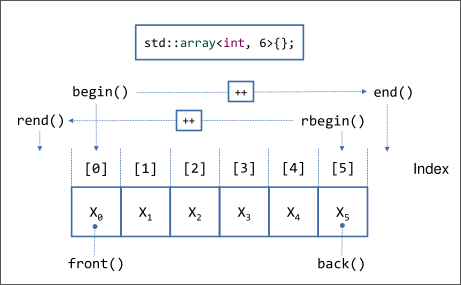
\includegraphics[scale=0.4]{2022-10-04-08_41_42.png}}[0.2,0.5]\\

\hline
\begin{lstlisting}
std::vector<int> arr{1,2,3,4,5};
std::vector arr{1,2,3,4,5}; 
//if elements are provided, then type can be omitted.
std::vector<int>(6); 
//int vector with size 6, with all elements being 0 -> default.
vector.push_back(element); //insert at end
vector.insert(pos,element); //insert at iterator
vector.erase(iterator); 
//vector.begin() vector.end()
vector.front();
vector.back();
vector.find(element);
\end{lstlisting}
& \minipg{Vector are simply the dynamic default datastructure in c++.\newline
\textbf{\textcolor{red}{Index variable type is unsigned int >> size\_t or std::vector<T>::size\_type}}\newline
\textbf{Iterating through a vector without at() is unsafe, \newline it will cause undefined behavior if out of bounds.\newline
With at() it will cause an exception instead.}}
{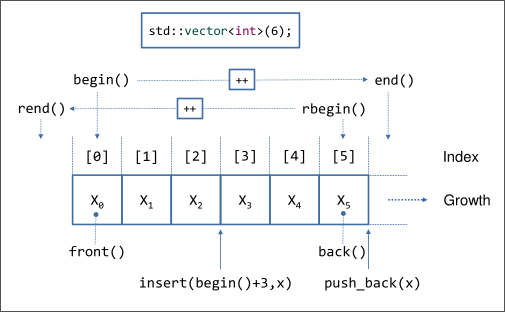
\includegraphics[scale=0.4]{2022-10-04-08_48_54.png}}[0.2,0.5]
\\

\hline
\begin{lstlisting}
[<capture>](<parameters>) -> <return-type> {
<statements>
}
\end{lstlisting}
& Basic Lambda syntax\newline
If you capture a value by value then it is by default const.\newline
 References, aka referenced pointer is handled with the \& symbol.\newline
 Note, capture and parameters are only different in one thing, capture is the state of the parent scope at compile time of the lambda, it therefore doesn't ever change, even if you change variables later on!\newline
\begin{lstlisting}
include <iostream>
using namespace std;

int main(int argc,char **argv)   {
    auto i=5;
    auto f = [=](int j) {cout<<"capture i="<<i<<", passing i as j="<<j<< endl; };
    while (i<30) {
        i += 10;
        f(i);
        // ambda capture i=5, passing i as argument j=1      
        // lambda capture i=5, passing i as argument j=25
        // lambda capture i=5, passing i as argument j=35
    } // i stays the same, even if we increment it!!!
}
\end{lstlisting}
\\
\hline
\begin{lstlisting}
auto zero_it = std::find(std::begin(v), std::end(v), 0);
if (zero_it == std::end(v)){
std::cout << "no zero found \n";
}
\end{lstlisting}
&

\\

\hline
\begin{lstlisting}
std::vector<int> v{5, 4, 3, 2, 1};
std::cout << std::accumulate(std::begin(v), std::end(v), 0)<< " = sum\n";

void printDistanceAndLength(std::string s) {
std::cout << "distance: "<< std::distance(s.begin(), s.end()) <<'\n';
std::cout << "in a string of length: "<< s.size()<<'\n';
}
\end{lstlisting}
& diverse standard library iteration and loops.
\\

\hline
\begin{lstlisting}
void print(int x) {
std::cout << "print: "<< x << '\n';
}
void printAll(std::vector<int> v) {
std::for_each(std::crbegin(v), std::crend(v), print);
}
\end{lstlisting}
& For each loop\\
\hline
\textbf{Function Overloading}\newline
\begin{lstlisting}
void incr(int & var);
void incr(int & var, unsigned delta);
\end{lstlisting}
& Will always use the more specific function.\newline
\textcolor{red}{Be aware that you should always make sure you enter the type that you want!\newline
Don't do automatic casting for overloaded functions!}\\
\hline
\end{tabular}
\end{table}
\pagebreak
\begin{table}[ht!]
\begin{tabular}{|m{0.2\linewidth}|m{0.755\linewidth}|}
\hline
\textbf{Default Values}\newline
\begin{lstlisting}
void incr(int & var, unsigned delta = 1);
void incr(int & var, unsigned delta) {
var += delta;
}
\end{lstlisting}
& \textcolor{teal}{Amazing functionality! This means that you can create \textbf{optional parameters!}}\\
\hline
\textbf{Alias}\newline
\begin{lstlisting}
using <alias> = <type>;
\end{lstlisting}
& Just don't do using namespace std;\\
\hline
\textbf{Lambda and std::function}\newline
\begin{lstlisting}
// std::function
std::function<double(double)>

// lambda 
auto some_func = [dependency](paremeter) {};
\end{lstlisting}
& Example for lambda:\newline
\begin{lstlisting}
int main() {
  double factor{3.0};
  auto const multiply = [factor](double value) {
    return factor * value;
  };
  applyAndPrint(1.5, multiply);
}

// create a new variable instead of capturing it
// can only be modified with mutable
// variable has type auto
auto squares = [x=1]() mutable {
std::cout << x *= 2;
};

// this pointer in lambda
struct S {
void foo() {
auto square = [this] {
member *= 2;
};
}
private:
int member{};
};
\end{lstlisting}
\, \newline
\textcolor{teal}{\char`\[  \char`\] These capture a variable from scope.}\newline
\textcolor{teal}{With brackets a variable can also be captured by reference -> \char`[ \&x\char`]}\newline
\textcolor{teal}{The \textcolor{red}{this} keyword can also be captured}\newline
\textcolor{teal}{\char`\( \char`\) These are for parameters just like a normal function}\\
\hline
\textbf{auto function return}\newline
\begin{lstlisting}
auto middle(std::vector<int> const& c) {
//check not empty
return c[c.size() / 2];
}
\end{lstlisting}
& This can automatically deduce the type, problem is,\newline
it might not show the type for every IDE.\newline
\textcolor{red}{The function body must be present for this!}\\
\hline
\textbf{Static} &
\textcolor{orange}{Static variables are essentially global variables, that are hidden behind a namespace. \newline
When defining a variable in the global scope, then it will NOT be linked to other files, unlike regular global variables.\newline
In functions, we can use static to define a variable that should keep its value after a change, even though we define the variable inside this function. This works as a static variable is always defined in the global scope with a different namespace to access it. \newline
This also means that \textbf{static variables are default initialized!}}\newline
\begin{lstlisting}
void spass() {
  static int x = 5;
  x++;
  std::cout << x << "\n";
}
\end{lstlisting}\\
\hline
\textbf{Inline} & 
\textcolor{orange}{Inline marks a function with a flag, that tells the compiler to consider this function possible to replace its calls directly.\newline
Replacing the calls simply mean instead of calling this function, place the function code in the calling function, reducing the amount of function calls in a program.\newline
It is important to know that the compiler would do this either way via optimization and that the inline keyword does not guarantee this behavior, it is simply a manual flag that tells the compiler to consider doing it.}\newline
\begin{lstlisting}
class Date {
int year, month, day;
public:
auto operator<(Date const& right) const -> bool;
};

inline auto operator>(Date const& left, Date const& right) -> bool {
  return right < left;
}
\end{lstlisting}\\
\hline
\end{tabular}
\end{table}
\pagebreak
\begin{table}[ht!]
\section{Best practices}
\begin{tabular}{|m{0.2\linewidth}|m{0.755\linewidth}|}
\hline
\textbf{Const by default} & 
\textcolor{red}{It is general best practice to always use const unless mutability is necessary!}\newline
\pic{2022-10-11-08_36_02.png}\\
\hline
\end{tabular}
\end{table}
\pagebreak
\begin{table}[h!]
\section{Default Operators}
\begin{tabular}{|m{0.2\linewidth}|m{0.755\linewidth}|}
\hline
\begin{lstlisting}
|| && == <= >= != > <
\end{lstlisting}
&
OR, AND, equals, smaller than or equals, greater than or equals, not equals, greater than, smaller than\\
\hline

\begin{lstlisting}
& | ^ >> <<
\end{lstlisting}
&
Bit operators.\\
\hline

\begin{lstlisting}
(5 > 4) ? true : false
\end{lstlisting}
&
Ternary Operator, or otherwise called inline if.\\
\hline
\end{tabular}
\section{Quirks}
\begin{tabular}{|m{0.25\linewidth}|m{0.705\linewidth}|}
\hline
\begin{lstlisting}
double f = 45 / 8;
\end{lstlisting}
&
In math operations the actual number takes precedence, here the numbers are int, therefore the value will be truncated to 5. If you want double or float division use 45.0 / 8.0 or 45.f / 8.f. \\
\hline
\textbf{\emph{Accessing Containers}} & 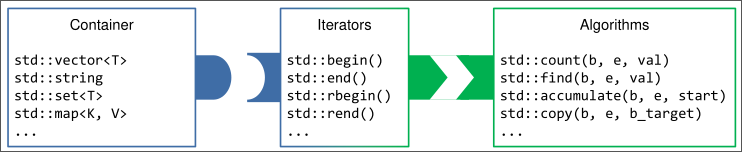
\includegraphics[scale=0.4]{2022-10-04-09_40_48.png}\\
\hline
\end{tabular}
\section{IO-Streams}
\begin{tabular}{|m{0.25\linewidth}|m{0.705\linewidth}|}
\hline
\begin{lstlisting}
std::ostream / std::istream
\end{lstlisting}
&
These represent the system IO, and they do therefore not have a value.\newline
This means you can't copy these, you can only pass references/pointers.
\\
\hline

\begin{lstlisting}
.clear() and .good()
\end{lstlisting}
&
If you use the streams yourself, aka not std::cout or std::cin, then you have to deal with the problems that can occur with it.\newline
This means that you have to check whether or not the stream is valid with .good() and clear it with .clear() should an error occur. \newline
Otherwise the stream will not be cleared for the next usage.
\\
\hline

\begin{lstlisting}
int inputAge(std::istream& in) {
    int age{-1};
    if (in >> age) {
        return age;
    }
    return -1;
}
\end{lstlisting}
&
Here the in >> age will return true if the input was successfully transferred into the stream.
\\
\hline
\textbf{\emph{\textcolor{red}{Terminating Inputstreams}}}
&
Terminating inputstreams can be done with \textbf{\emph{\textcolor{red}{CTRL+D}}}\\
\hline
Stream states & \vspace{2mm}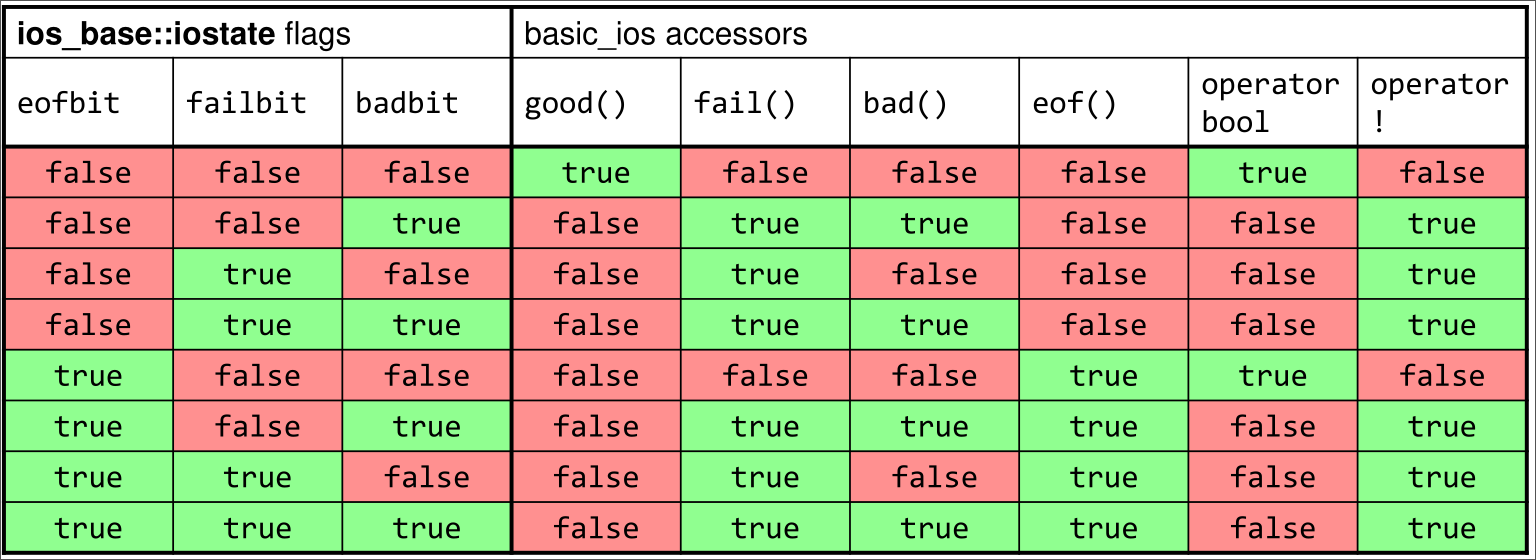
\includegraphics[scale=0.25]{2022-10-04-08_13_36.png} \\
\hline
\emph{Formatting} &
\vspace{2mm}
\begin{itemize}
  \item std::cout << std::oct << number;
  \item std::cout << std::hex << number;
  \item std::cout << std::dec << number;\newline
    \textcolor{red}{These are sticky, meaning this formatting will stick from that line on.}\newline
  \item std::setprecision 
  \item std::fixed 
  \item std::scientific
  \item std::left
  \item std::setw(10) //output at least 10 digits long
\vspace{-3mm}
\end{itemize}
\\
\hline
\end{tabular}
\section{Loops}
\begin{tabular}{|m{0.25\linewidth}|m{0.705\linewidth}|}
\hline
\textbf{\emph{Range based for-loop}} &
\vspace{2mm}
\begin{lstlisting}
for(const& elem : vec ) {
  std::cout << elem << "\n";
}
\end{lstlisting}\\
\hline
\textbf{\emph{Iterator based for-loop}}
& \minipg{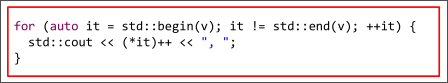
\includegraphics[scale=0.4]{2022-10-04-09_24_39.png}\newline non constant}
{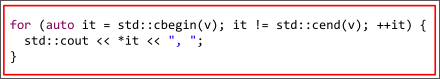
\includegraphics[scale=0.4]{2022-10-04-09_24_44.png}\newline constant}[0.4,0.5]\\
\hline
\end{tabular}
\end{table}
\pagebreak
\begin{table}[ht!]
\section{Pointer and References}
\begin{tabular}{|m{0.2\linewidth}|m{0.755\linewidth}|}
\hline
\textbf{Returning References}\newline
\begin{lstlisting}
// ok
std::ostream & sayHello(std::ostream & out) {
return out << "Hello";
}

// No 
std::string & create() {
std::string name{"John"};
return name;
}
\end{lstlisting}
& 
You can return references, but keep in mind that this basically means returning a pointer.\newline
If you create a variable and return a reference to it, then that pointer is now invalid!\newline
\textcolor{red}{Accessing an invalid pointer will cause a segmentation fault!}\\
\hline
\end{tabular}
\begin{tabular}{|m{0.2\linewidth}|m{0.755\linewidth}|}
\hline

\hline
\end{tabular}
\section{Cmake}
\begin{tabular}{|m{0.2\linewidth}|m{0.755\linewidth}|}
\hline
\textbf{ClangD LSP include} & 
In order to include your projects in the clanD server, you need to compile a json file with cmake.\newline
\large\textbf{\textcolor{teal}{cmake -DCMAKE\_EXPORT\_COMPILE\_COMMANDS=1}}\newline
\normalsize After this command everything will be setup for your to start programming with all the whistles that you need.\\
\hline
\end{tabular}
\section{Error Handling}
\begin{tabular}{|m{0.2\linewidth}|m{0.755\linewidth}|}
\hline
\textbf{Ways to handle Errors} &
\vspace{2mm}
\begin{enumerate}
  \item Ignore the error and provide a potentially \textcolor{red}{undefined behavior}
  \item Return a \textcolor{red}{standard result} to cover the error
  \item Return an \textcolor{red}{error code} or error value
  \item Provide an \textcolor{red}{error status} as a side-effect
  \item Throw an \textcolor{red}{exception} -> perfomance heavy
\end{enumerate}\\
\hline
Ignoring an error & 
Example\newline
\begin{lstlisting}
std::vector v{1, 2, 3, 4, 5};
v[5] = 7;
\end{lstlisting}
\, \newline
\begin{itemize}
  \item Relies on the caller to satisfy all preconditions
  \item Viable only if not dependent on other resources
  \item Most efficient implementation\newline
   No unnecessary checks
  \item Simple for the implementer but harder for the caller
  \item Should be done consciously and consistently!
\end{itemize}
\\
\hline
Cover an Error & 
\begin{lstlisting}
int div(int number, int number2) {
  if(number2 == 0) {
    return 0;
  }
  return number / number2;
}
\end{lstlisting}
\, \newline
This is bad as it can lead to strange behavior in debugging, but is performant!\\
\hline
Error Value with std::optional & 
\begin{lstlisting}
std::optional<std::string> inputName(std::istream & in) {
  std::string name{};
  if (in >> name) return name;
  return {};
}
\end{lstlisting}
\, \newline
\textcolor{teal}{This simply returns the type string if name was able to be parsed, or no type, aka void if it could not be parsed.}\\
\hline
Error Status Side Effect &

\\
\hline
Exceptions & 
\begin{lstlisting}
throw std::some_exception{"error text"};
throw ExceptionName;
throw ENUM;

// don't
throw 2;
throw "sowwy ewwow";
\end{lstlisting}
\, \newline
With C++ you can throw all kinds of crap, but please, throw exceptions or enums.\\
\hline
\end{tabular}
\end{table}
\pagebreak
\begin{table}[ht!]
\section{Classes and Structs}
\begin{tabular}{|m{0.2\linewidth}|m{0.755\linewidth}|}
\hline
Classes &
\textcolor{orange}{Classes and Structs are defined like this:}\newline
\begin{lstlisting}
class Something { 
public:
// default for struct
// visible for everyone
static int returnValue();
// static simply means that you can use this function without an instance!
protected:
// visible only to class and subclasses
private:
// default for classes
// visible only for class
};
\end{lstlisting}
\, \newline
\textcolor{teal}{Other than the private and public denotations, structs are defined the same way, and also operate the same way!}\\
\hline
\textbf{Initializer List\newline and Constructor} &
\textcolor{purple}{The simple difference with initializer lists to the java way of initializing objects, is that with initializer lists, you only create an object once, when doing it in the java way you create two objects, meaning that you will lose performance!}\newline
\begin{lstlisting}
class Something {
private:
  int a,b;
public:
  Something(int a, int b);
}

Something(int a, int b) : 
a{a}, b{b} {
// regular constructor
// !! a constructor doesn't return a value !!
}
\end{lstlisting}
\, \newline
\textcolor{teal}{C++ has a default constructor -> Something()}\newline
\textcolor{orange}{\textbf{A constructor does not return a value!}}\\
\hline
\textbf{Copy and Move Constructor} & 
\begin{lstlisting}
Date d{};
Date d2{d};
// copies d into d2
// 2 instances now!
Date d3{std::move(d)};
// move constructor!
// this moves the values of d into d3, 1 instance only!
\end{lstlisting}
\, \newline
\begin{lstlisting}
Date() = default; // default constructor, if you write this, write default to avoid overwriting it!
Date(Date const&); // copy constructor
Date(Date &&); // move constructor
\end{lstlisting}
\\
\hline
\textbf{default values in Constructors} & 
\begin{lstlisting}
explicit Date(int year, int month = 1, int day = 1);
// explicit means that we do not want implicit conversion -> double to int
// We can now call this constructor with either 1, 2 or 3 parameters, as 2 of them have a default value!
\end{lstlisting}
\\
\hline
List Constructor with Containers & 
\begin{lstlisting}
std::vector(5,10);
// creates a vector with 5 elements of value 10!
// same as -> std::vector(std::initializer_list<5> 10);

std::vector{5,10};
// creates a vector with element 5 and 10!
\end{lstlisting}\\
\hline
\textbf{Destructor} & 
\begin{lstlisting}
~Date();
// do something before we delete this instance
\end{lstlisting}
\, \newline
\textcolor{orange}{\textbf{This may never throw an exception!}}\\
\hline
\textbf{Inheritance} & 
\begin{lstlisting}
class SubDate : public Date { 
// public -> keep as is
// protected -> change all public to protected -> not directly accessible
// private -> change all inherited to private -> not directly accessible
// default inheritance is based on class or strcut -> private and public
};

class SubDate2 : public SubDate, public Date {
// ...
};
\end{lstlisting}
\, \newline
\textcolor{teal}{A class can inherit from 1 \textbf{OR MORE} classes!}\\
\hline
\textbf{Scope} & 
\textcolor{orange}{Scope is denoted with the :: operators -> Calculator::negate(); \newline call the static function negate form Calculator}\\
\hline
Calling SuperClass Constructors & 
\begin{lstlisting}
Something() : ParentOfSomething() {
/ ...
}
// or you can call another constructor of the same element!
Something() : Something() {
/ ...
}
\end{lstlisting}
\, \newline
\textcolor{orange}{Unlike java, here we can just call constructors of multiple parent classes!}\\
\hline
const this & 
\textcolor{orange}{\textbf{The this keyword can be const, it may then not change the values of membervariables!}}\\
\hline 
\end{tabular}
\end{table}
\pagebreak
\begin{table}[ht!]
\begin{tabular}{|m{0.2\linewidth}|m{0.755\linewidth}|}
\hline
static functions & 
Static functions are just in the namespace of the class, they can't access or call any object dependent code/variables, and can only use the static variables in the class.\newline
They are usually used to provide extra functionality, that has nothing to do with the specific instance, but still makes sense to bundle with that class as it has related functionality.\newline
\begin{lstlisting}
class globi {
  static void something() {
      std::cout << "useless function" << "\n";
  }
};

int main() { 
  globi::something(); // ok static
}
\end{lstlisting}\\
\hline
\textbf{static variables in classes} &
\textcolor{purple}{Static variables in classes are considered to be global with a special namespace, just like regular static variables.\newline
The only difference is that this static variable is the same for \textbf{every instance of this class}, meaning that this will be a \textbf{shared state} between all classes.}
\begin{lstlisting}
static const Date myDate;
// this is an immutable global variable that can be accessed (read-only) with SomeThing::myDate;
static Date myOtherDate;
// this can be accessed and also changed, it is a mutable global variable!!
\end{lstlisting}\\
\hline
\end{tabular}
\section{Operator Overloading}
\begin{tabular}{|m{0.2\linewidth}|m{0.755\linewidth}|}
\hline
Operators &
\vspace{2mm}
\minipg{
Overloadable:\newline
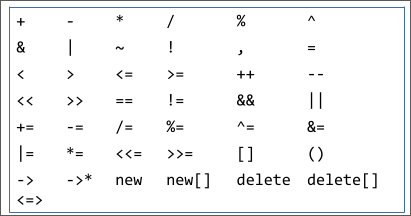
\includegraphics[scale=0.35]{2022-10-18-09_26_28.png}
}{
Not Overloadable:\newline
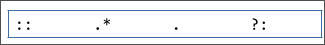
\includegraphics[scale=0.4]{2022-10-18-09_26_34.png}
}[0.3,0.5]\\
\hline
Spaceship Operator &
\textcolor{orange}{The spaceship operator implements the usual comparison operators for you class\newline
This means <, >, <=, >=,== ,!=}\newline
\begin{lstlisting}
class Date {
int year, month, day;
public:
auto operator<=>(Date const& right) const -> std::strong_ordering {
  if (year != right.year) {
    return year <=> right.year;
  }
  if (month != right.month) {
    return month <=> right.month;
  }
  return day <=> right.day;
}
auto operator==(Date const& right) const -> bool {
return (*this <=> right) == std::strong_ordering::equal;
} //Also allows != comparison
};
\end{lstlisting}
\, \newline
\textcolor{red}{Since C++ 20 you can also use the following to default the <=> operator}\newline
\begin{lstlisting}
class Date {
int year, month, day;
public:
auto operator<=>(Date const& right) const = default;
};
\end{lstlisting}
\\
\hline
Defaulting Operator & 
Just like with the <=> Operator you can default other operators: \newline
\begin{lstlisting}
class Point {
int x, y;
public:
auto operator==(Date const& right) const = default;
};
\end{lstlisting}\\
\hline
\textbf{Strong Ordering with <=>} \newline
defined in: <functional>&
\textcolor{teal}{Usually used with ints or Dates}\newline
\textcolor{red}{\textbf{All values are indistinguishable}}\newline
\textcolor{orange}{\textbf{one of: a > b, a == b, a < b must be true}}\newline
\begin{lstlisting}
auto operator<=>(Date const& right) const -> std::strong_ordering;
\end{lstlisting}
\, \newline
A list of possibilities:\newline
\begin{itemize}
  \item \textcolor{teal}{std::strong\_ordering::less} \,\,-> a < b 
  \item \textcolor{teal}{std::strong\_ordering::equal}\,\,-> a == b 
  \item \textcolor{teal}{std::strong\_ordering::greater}\,-> a > b 
  \vspace{-3mm}
\end{itemize}\\
\hline
\textbf{Weak Ordering with <=>}\newline
defined in: <functional> & 
\textcolor{teal}{Usually used with words, -> case insenstivive -> hello == Hello}\newline
\textcolor{red}{\textbf{All values may be distinguishable}}\newline
\textcolor{orange}{\textbf{one of: a > b, a == b, a < b must be true}}\newline
\begin{lstlisting}
auto operator<=>(Date const& right) const -> std::weak_ordering;
\end{lstlisting}
\, \newline
A list of possibilities:\newline
\begin{itemize}
  \item \textcolor{teal}{std::weak\_ordering::less} \,\,-> a < b 
  \item \textcolor{teal}{std::weak\_ordering::equivalent}\,\,-> a == b 
  \item \textcolor{teal}{std::weak\_ordering::greater}\,-> a > b 
  \vspace{-3mm}
\end{itemize}\\
\hline
\end{tabular}
\end{table}
\pagebreak
\begin{table}[ht!]
\begin{tabular}{|m{0.2\linewidth}|m{0.755\linewidth}|}
\hline
\textbf{Partial Ordering with <=>} \newline
defined in: <functional>&
\textcolor{teal}{Usually used with values that can be something like NaN!}\newline
\textcolor{red}{\textbf{All values may be distinguishable}}\newline
\textcolor{orange}{\textbf{a > b, a == b , a < b can all be false}}\newline
\begin{lstlisting}
auto operator<=>(Date const& right) const -> std::partial_ordering;
\end{lstlisting}
\, \newline
A list of possibilities:\newline
\begin{itemize}
  \item \textcolor{teal}{std::partial\_ordering::less} \,\,-> a < b 
  \item \textcolor{teal}{std::partial\_ordering::equivalent}\,\,-> a == b 
  \item \textcolor{teal}{std::partial\_ordering::greater}\,-> a > b
  \item \textcolor{teal}{std::partial\_ordering::unordered}\,-> none of the above
  \vspace{-3mm}
\end{itemize}\\
\hline
Inline Operator &
\textcolor{orange}{The best way to define an operator is with the inline version:}\newline
\begin{lstlisting}
class Date {
    int year, month, day;
  public:
    auto print(std::ostream & os) const -> std::ostream& {
    //print logic
    }
};
Inline auto operator<<(std::ostream & os, Date const& date) -> std::ostream& {
  return date.print(os);
}
\end{lstlisting}
\, \newline
\textcolor{teal}{This makes sure that the operator function that is outside of your class can have any order of variables -> inside the class it would always be the "this" keyword first.\newline
However it also makes sure that the operator function respects the private variables -> no access since outside of class}\\
\hline
+= and + &
\textcolor{orange}{Since you can have 2 different implementation of + and +=, you have to make sure they actually have the same functionality!}\newline
\begin{lstlisting}
struct Ring5 : boost::addable<Ring5> {
  auto operator*=(Ring5 const&r) -> Ring5 {
  val = (val * r. val) % 5;
  return *this;
  }
};
inline auto operator*(Ring5 l, Ring5 const& r) -> Ring5 {
  return l += r;
}
\end{lstlisting}\\
\hline
Automatic conversion & 
\textcolor{orange}{You can also use the operators to convert to unsigned etc.\newline
This is worse than a static cast, but it requires less code}\newline
\begin{lstlisting}
struct Ring5 {
  Ring5(unsigned x) : val{x % 5} {}
    operator unsigned() const { // convert to unsigned
    return val;
  }
};
\end{lstlisting}\\
\hline
\end{tabular}
\section{Namespaces}
\begin{tabular}{|m{0.2\linewidth}|m{0.755\linewidth}|}
\hline
Global Namespace & 
\textcolor{orange}{The global namespace -> "::" is usually omitted, as it is usually unique, keep it that way please!}\newline
\begin{lstlisting}
::std::string x = "ping"; // with global namespace
std::string y = "pang"; // without global namespace
\end{lstlisting}\\
\hline
Accessing Namespace & 
\begin{lstlisting}
std::string x = "ping";
// the namespace is std, with the class to access being string.
\end{lstlisting}\\
\hline
Creating Namespace & 
\textcolor{teal}{Namespaces are made similarly to classes, but without the curly braces at the end!\newline
We also do not have a "this" keyword here, obviously!}\newline
\begin{lstlisting}
namespace gurri {
  void somefunc();
  int someotherfunc();
}
\end{lstlisting}
\, \newline
\textcolor{orange}{Just like classes, namespaces are defined in the hpp, or h file for code style purposes!}\\
\hline
Using directive & 
\textcolor{orange}{The using directive should only ever be explicitly used.\newline
This means don't use the entire namespace, only use specific functions that you know will not be overwritten again!}\newline
\begin{lstlisting}
using std::string; // ok if no other package is used for string
string x = "ping"; // ok

using namespace std; // NO FUCK OFF!
\end{lstlisting}\\
\hline
Anonymous Namespaces & 
\textcolor{orange}{These namespaces are used to hide implementation details from other files.\newline
The reason is essentially that no-one can access this namespace as it has no name.}\newline
\begin{lstlisting}
namespace{
  void print() {
    std::cout << "pingpang\n";
  }
  print(); // ok
}
print(); // ERROR, no access to print!
\end{lstlisting}\\
\hline
\end{tabular}
\end{table}
\pagebreak
\begin{table}[ht!]
\begin{tabular}{|m{0.2\linewidth}|m{0.755\linewidth}|}
\hline
Argument Dependent Lookup & 
\vspace{2mm}
\begin{lstlisting}
namespace lol {
  struct type_one {};
  auto f(type_one) -> void {
    std::cout << "this is bs\n";
  }
}
namespace lmao {
  struct type_two {};
  auto f(type_two) -> void { std::cout << "This is the other bs\n"; }
  auto h(lol::type_one) -> void { std::cout << "No worky 1\n"; }
  auto g(lol::type_one) -> void { std::cout << "No worky 2\n"; }
}
auto g(lmao::type_two) -> void { std::cout << "this one worky\n"; }
int main() {
  lol::type_one t1{};
  f(t1); // implicit call to namespace lol
  lmao::type_two t2{};
  f(t2); // implicit call to namespace lmao
  // h(t2); no worky, t1 has no access to namespace lmao
  lmao::g(t1); // works as it is called explicitly!
  //g(t1); trying to use the g function from lmao, but it can't find it!
  // you can't do argument dependent lookup across 2 namespaces, this only works with 1 namespace!
  // h(t1); aka, this also won't work, you need to use the lmao:: before the function for it to work
  // Simply put, just do not depend on this crap and write lol or lmao when you want to use these functions ....
  g(t2); // ok, calls the global function as this is the most specific one
  return 0;
}
\end{lstlisting}
\\
\hline
Overwriting the std Namespace & 
\textcolor{orange}{Overwriting the standard namespace is not allowed!\newline
If you want to overwrite something in the std namespace use this workaround:}\newline
\begin{lstlisting}
using std::ostream;
using std::vector;
using out = std::ostream_iterator<int>;

namespace X { // create a namespace to use instead of the std vector
  struct vec : vector<int> { // vec is a new type
  using vector<int>::vector; // inherit ctors
};
// this is now allowed!!:
auto operator<<(ostream& os, vec const& v) -> ostream& { 
  copy(begin(v), end(v), out{os, ","});
  return os;
}
}
auto print(ostream& os) -> void {
  // copy all vector members to ostream and print them!
  using outv = std::ostream_iterator<X::vec>;
  vector<X::vec> vv{{1, 2, 3}, {4, 5, 6}};
  copy(begin(vv), end(vv), outv{os, "\n"});
}
\end{lstlisting}\\
\hline
\end{tabular}
\section{Enums}
\begin{tabular}{|m{0.2\linewidth}|m{0.755\linewidth}|}
\hline
Scopend and Unscoped Enums &
\textcolor{orange}{The difference is only the use of scope and the cast.}\newline
\begin{lstlisting}
// unscoped:
enum Day { 
  Mon, Tue, Wed, Thu, Fri, Sat, Sun
}; // 0, 1, 2, 3, 4, 5, 6
// conversion to int:
int day = Sun; // ok

// scoped:
enum class Day { 
  Mon, Tue, Wed, Thu, Fri, Sat, Sun
}; // 0, 1, 2, 3, 4, 5, 6
// conversion to int:
int day = Sun; // ERROR!
int day = static_cast<int>(Day::Sun); // ok

// Note, the scoped enum always requires the scope operator
auto test(Day day) {
  if (day == Day::Sun) { // scope used here, no scope for the regular enum!
    return true;
  }
  return false;
}
\end{lstlisting}\\
\hline
Int to Enum & 
\textcolor{orange}{Converting from int to enum always needs a cast:}\newline
\begin{lstlisting}
DayOfWeek tuesday = static_cast<DayOfWeek>(1);
\end{lstlisting}\\
\hline
Values for Enums &
\textcolor{teal}{You can specify the number for each part of an enum}\newline
\begin{lstlisting}
enum FilePermissions {
  readable = 1,  //001
  writeable = 2, //010
  executable = 4 //100
};
\end{lstlisting}\\
\hline
\end{tabular}
\end{table}
\pagebreak
\begin{table}[ht!]
\begin{tabular}{|m{0.2\linewidth}|m{0.755\linewidth}|}
\hline
Specifying Types & 
\textcolor{orange}{You can specify a type for an enum to use:}\newline
\begin{lstlisting}
enum LaunchPolicy : unsigned char {
sync = 1,
async = 2,
gpu = 4
}
\end{lstlisting} 
\, \newline
\textcolor{teal}{\textbf{Keep in mind that it will still have to be an integral type!!}}\\
\hline
Enum Operator Overloading & 
\begin{lstlisting}
enum DayOfWeek {
  Mon, Tue, Wed, Thu, Fri, Sat, Sun
};
auto operator++(DayOfWeek& d) -> DayOfWeek { // prefix
  return static_cast<DayOfWeek>((aday + 1) % (Sun + 1));
}
auto operator++(DayOfWeek& d, int) -> DayOfWeek { // postfix
  return static_cast<DayOfWeek>((aday + 1) % (Sun + 1));
}
\end{lstlisting}\\
\hline
\end{tabular}
\section{Containers}
\begin{tabular}{|m{0.2\linewidth}|m{0.755\linewidth}|}
\hline
Categories &
\vspace{2mm}
\begin{itemize}
\item \textcolor{orange}{Sequence Containers: \newline
  Elements are accessible in order as they were inserted/created\newline
  find in linear time through algorithm find}
\item \textcolor{orange}{Associative Containers:\newline
  Elements are accessible in sorted order\newline
  find as member function in logrithmic time}
\item \textcolor{orange}{Hashed Container (Unsorted Associative Container)\newline
  Element are accessible in unspecified order\newline
  find as member function in constant time}
\vspace{-2mm}
\end{itemize}\\ 
\hline
General Container Info &
\vspace{2mm}
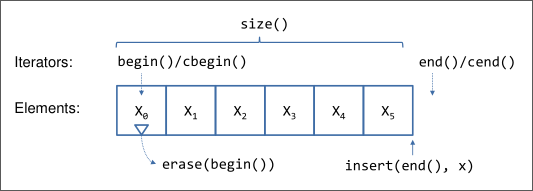
\includegraphics[scale=0.4]{2022-11-08-08_23_10.png}\newline
\begin{itemize}
\item \textcolor{orange}{begin()/end()}: Get iterators for algorithms and iteration in general
\item \textcolor{orange}{erase(iter)}: Removes the element at position the iterator iter points to
\item \textcolor{orange}{insert(iter, value)}: Inserts value at the position the iterator iter points to
\item \textcolor{orange}{size()/empty()}: Check the size of the container
\vspace{-2mm}
\end{itemize}
\, \newline
\textcolor{teal}{Containers can be:}\newline
\begin{itemize}
  \item \textcolor{teal}{default-constructed}: std::vector<int> v{}
  \item \textcolor{teal}{copy-constructed}: std::vector<int> v2{v};
\item \textcolor{teal}{Equality compared if the same type}: if(v == v2)
\item \textcolor{teal}{lexicographically compared if elements can be compared}
\item \textcolor{teal}{emptied with clear()}
\vspace{-2mm}
\end{itemize}\\
\hline
Initialization & 
\textcolor{orange}{Just like vectors, containers can usually be initialized via the 3 main methods: }\newline
\begin{itemize}
  \item \textcolor{teal}{initializer list}: std::vector<int> v{1,2,3,5,6};
  \item \textcolor{teal}{Construction with number of elements}: std::vector<int> v(5, 10);
  \item \textcolor{teal}{With range}: std::vector<int> v{cbegin(v), cend(v)};
\item \textcolor{teal}{item 4}
\vspace{-2mm}
\end{itemize}\\
\hline
Sequence Containers & 
\vspace{2mm}
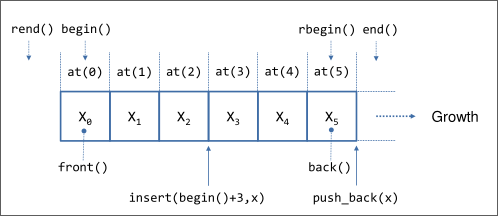
\includegraphics[scale=0.4]{2022-11-08-08_32_12.png}\newline
\begin{itemize}
\item \textcolor{teal}{std::vector}
\item \textcolor{teal}{std::deque}
\item \textcolor{teal}{std::list}
\item \textcolor{teal}{std::array}
\vspace{-2mm}
\end{itemize}\\
\hline
std::array \newline
defined in: <array> &
\vspace{2mm}
\begin{lstlisting}
std::array values{1,2,3,5,6};
// instead of
int obsolete[]{2,3,4,5,6};
\end{lstlisting}
\, \newline
\begin{itemize}
\item \textcolor{orange}{Fixed-size container, can't insert/append}
\item \textcolor{orange}{Can be initialized at compile time}
\item \textcolor{orange}{use std::array over C style array}
\item \textcolor{orange}{item 4}
\vspace{-2mm}
\end{itemize}\\ 
\hline
\end{tabular}
\end{table}
\pagebreak
\begin{table}[ht!]
\begin{tabular}{|m{0.2\linewidth}|m{0.755\linewidth}|}
\hline
Double Ended queue std::deque \newline 
defined in: <deque>& 
\vspace{2mm}
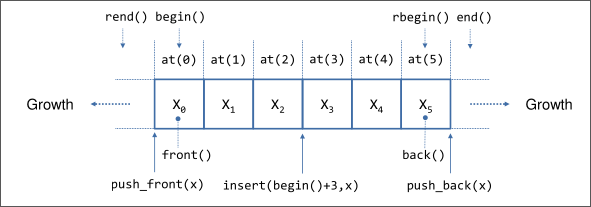
\includegraphics[scale=0.4]{2022-11-08-08_39_23.png}\newline
\textcolor{orange}{This is like the std::vector with the additional functions: \textbf{push\_front() and pop\_front()}}\newline
\textcolor{teal}{Special implementation for std::vector<bool> and std::deque<bool>.}\\
\hline
std::list \newline 
defined in: <list> & 
\vspace{2mm}
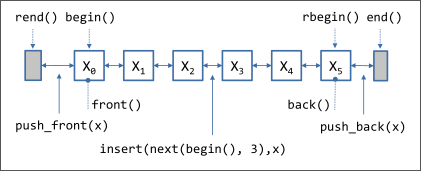
\includegraphics[scale=0.4]{2022-11-08-08_41_00.png}\newline
\begin{itemize}
\item \textcolor{orange}{Efficient insertion in any position}
\item \textcolor{orange}{Lower efficiency in bulk operations}
\item \textcolor{orange}{Requires member-function call for sort() etc}
\item \textcolor{orange}{Only bi-directional iterators - no index access!}
\vspace{-2mm}
\end{itemize}\\
\hline
std::forward\_list \newline 
defined in: <forward\_list> & 
\begin{lstlisting}
std::forward_list<int> l{1, 2, 3, 4, 5, 6};
\end{lstlisting}
\, \newline
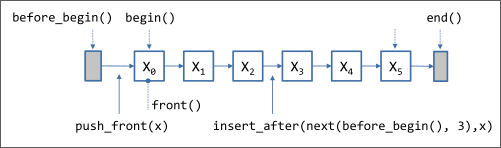
\includegraphics[scale=0.4]{2022-11-08-08_43_38.png}\newline
\begin{itemize}
\item \textcolor{orange}{Efficient insertion AFTER any position, but clumsy with iterator to get "before position"}
\item \textcolor{orange}{Only forward-iterators, lumsy to search and remove, use member-functions not algorithms}
\item \textcolor{orange}{Avoid, except when there is a specific need! \textbf{Better use std::list or std::vector}}
\vspace{-2mm}
\end{itemize}\\
\hline
std::stack \newline 
defined in: <stack> & 
\begin{lstlisting}
std::stack<int> s{};
s.push(42);
std::cout << s.top();
s.pop();
\end{lstlisting}
\, \newline
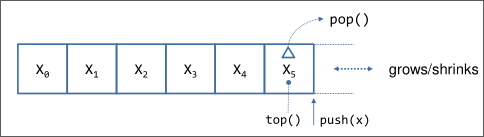
\includegraphics[scale=0.4]{2022-11-08-08_47_04.png}\newline
\begin{itemize}
\item \textcolor{orange}{Uses std::deque or std::vector/std::list and limits its functionality to stack operation}
\item \textcolor{orange}{No iteration}
\item \textcolor{orange}{Delegates push\_back(), back() and pop\_back()}
\item \textcolor{orange}{No longer a proper container, \textbf{deliberate limitation!}}
\vspace{-2mm}
\end{itemize}\\
\hline
std::queue  \newline 
defined in: <queue> & 
\begin{lstlisting}
std::queue<int> q{};
q.push(42);
std::cout << q.front();
q.pop();
\end{lstlisting}
\, \newline
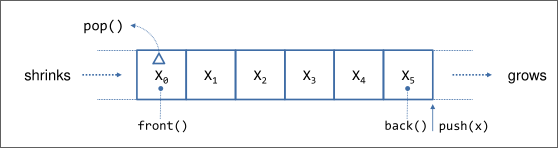
\includegraphics[scale=0.4]{2022-11-08-08_48_42.png}\newline
\begin{itemize}
\item \textcolor{orange}{Uses std::deque or std::vector/std::list and limits its functionality to stack operation}
\item \textcolor{orange}{No iteration}
\item \textcolor{orange}{Delegates push\_back(), back() and pop\_back()}
\item \textcolor{orange}{No longer a proper container, \textbf{deliberate limitation!}}
\vspace{-2mm}
\end{itemize}\\
\hline
std::priority\_queue & 
\begin{lstlisting}
std::priority_queue<int> q{};
q.push(42);
std::cout << q.front();
q.pop();
\end{lstlisting}
\, \newline
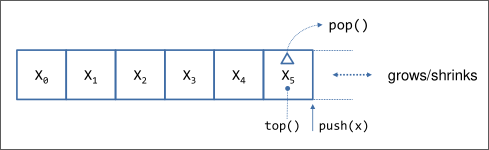
\includegraphics[scale=0.4]{2022-11-08-08_51_40.png}\newline
\begin{itemize}
\item \textcolor{orange}{Uses std::deque or std::vector/std::list and limits its functionality to stack operation}
\item \textcolor{orange}{No iteration}
\item \textcolor{orange}{Delegates push\_back(), back() and pop\_back()}
\item \textcolor{orange}{No longer a proper container, \textbf{deliberate limitation!}}
\item \textcolor{orange}{Keeps elements sorted}
\item \textcolor{orange}{top() element is always the smallest (requires elment type to be comparable)}
\vspace{-2mm}
\end{itemize}\\
\hline
\end{tabular}
\end{table}
\pagebreak
\begin{table}[ht!]
\begin{tabular}{|m{0.2\linewidth}|m{0.755\linewidth}|}
\hline
Associative Containers & 
\vspace{2mm}
\begin{itemize}
\item \textcolor{Orange}{Key Unique / Key only: std::set}
\item \textcolor{Orange}{Key Unique / Key and value: std::map}
\item \textcolor{Orange}{Multiple Equivalent Keys / Key only: std::multiset}
\item \textcolor{Orange}{Multiple Equivalent Keys / Key and value: std::multimap}
\vspace{-2mm}
\end{itemize}\\ 
\hline
std::set \newline 
defined in: <set> &
\begin{lstlisting}
std::set<int> values{5,6,2,9,8};
\end{lstlisting}
\, \newline
\begin{itemize}
\item \textcolor{orange}{Stores elements in sorted order (\textbf{ascending by default})}\newline
  order can be overwritten by the 2nd template parameter
\item \textcolor{orange}{Iteration walks over the elements in order}\newline
  Keys cannot be modified through iterators!
\item \textcolor{orange}{Use member functions for .find and .count}\newline
  Tree-search instead of sequential search\newline
  Result of .count(element is either 0 or 1\newline
  Since C++20 there is a .contains(element) member
\item \textcolor{orange}{Initializer does not need to be sorted}\newline
  s.contains(x) as quick check if x is present in std::set
\item \textcolor{orange}{Discouraged alternatives: s.find(x) != s.end() or s.count(x)}
\vspace{-2mm}
\end{itemize} 
\, \newline
\textcolor{orange}{Example:}\newline
\begin{lstlisting}
#include <iostream>
#include <set>
auto filterVowels(std::istream& in, std::ostream& out) -> void {
  std::set const vowels{'a', 'e', 'o', 'u', 'i', 'y'};
  char c{};
  while (in >> c) {
    if (!vowels.contains(c)) {
      out << c;
    }
  }
}
auto main() -> int {
  filterVowels(std::cin, std::cout);
}
\end{lstlisting}\\
\hline
std::map  \newline 
defined in: <map> &
\begin{lstlisting}
std::map<char, size_t> vowels{{'a', 3}, {'e', 8}, {'i', 5}, {'o', 4}, {'u', 2}, {'y', 1}};
\end{lstlisting}
\, \newline
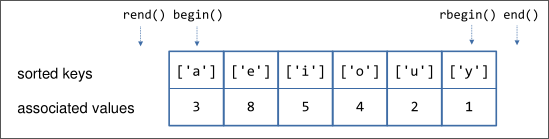
\includegraphics[scale=0.4]{2022-11-08-09_15_15.png}\newline
\begin{itemize}
\item \textcolor{Orange}{Stores key-value pairs in sorted order}\newline
  Sorted by key in ascending order\newline
  \textcolor{teal}{Order can be overwritten by the 3rd template parameter}
\item \textcolor{Orange}{Iterators access std::pair<key, value>}\newline
  Use .first for key and .second for value
\item \textcolor{orange}{m.contains(x) as quick check if x is a key present in std::map}\newline
  Discouraged alternative m.find(x) != m.end() or m.count(x)
\item \textcolor{orange}{auto is simpler than std::pair<key, value>, obviously lol}
\item \textcolor{orange}{Indexing operator[] inserts a new entry automatically if key is not present}\newline
  Key is the argument of the index operator, values is the default value of the value type\newline
  Returns the value by reference, which allows modification
\vspace{-2mm}
\end{itemize} 
\, \newline
\textcolor{orange}{Example:}\newline
\begin{lstlisting}
auto countVowels(std::istream& in, std::ostream& out) -> void {
  std::map<char, size_t> vowels{{'a', 0}, {'e', 0}, {'i', 0}, {'o', 0}, {'u', 0}, {'y', 0}};
  char c{};
  while (in >> c) {
    if (vowels.contains(c)) { // only count those chars that are already in the map
    ++vowels[c];
    for_each(cbegin(vowels), cend(vowels), [&out](auto const& entry) {
      // entry is a pair<char, size_t>
      out << entry.first << " = "<< entry.second << '\n';
    });
  }
}
\end{lstlisting}\\
\hline
std::multiset and std::multimap \newline
defined in <set> and <map> respectively& 
\begin{lstlisting}
std::multiset<char> letters{'a', 'a', 'c', 'c', 'c', 'e', 'e', 'f'};
// note the c that appears 3 times!
\end{lstlisting}
\, \newline
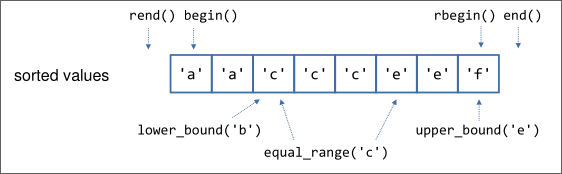
\includegraphics[scale=0.4]{2022-11-08-09_24_23.png}\newline
\begin{itemize}
\item \textcolor{orange}{Multiple Keys allowed}\newline
  Use equal\_range() or lower\_bound()/upper\_bound() member functions/algorithms to find boundaries of equivalent keys
\item \textcolor{orange}{Can be a bit more tedious to work with than std::set}
\vspace{-2mm}
\end{itemize} \\
\hline
\end{tabular}
\end{table}
\pagebreak
\begin{table}[ht!]
\begin{tabular}{|m{0.2\linewidth}|m{0.755\linewidth}|}
\hline
&
\textcolor{orange}{Example:}\newline
\begin{lstlisting}
auto sortedStringList(std::istream& in, std::ostream& out) -> void {
  using inIter = std::istream_iterator<std::string>;
  using outIter = std::ostream_iterator<std::string>;
  std::multiset<std::string> words{inIter{in}, inIter{}};
  copy(cbegin(words), cend(words), outIter(out, "\n"));
  auto current = cbegin(words);
  while (current != cend(words)) {
    auto endOfRange = words.upper_bound(*current);
    copy(current, endOfRange, outIter{out, ", "});
    out << '\n'; // next range on new line
    current = endOfRange;
  }
}
\end{lstlisting} 
\, \newline
\begin{itemize}
\item \textcolor{orange}{First copy-algorithm call prints each word on separate line}
\item \textcolor{orange}{Code in while-loop groups equivalent words on one line}
\vspace{-2mm}
\end{itemize} \\
\hline
std::unordered\_set \newline 
defined in: <unordered\_set>& 
\begin{lstlisting}
#include <algorithm>
#include <iostream>
#include <iterator>
#include <unordered_set>
auto main() -> int {
  std::unordered_set<char> const vowels{'a', 'e', 'i', 'o', 'u'};
  using in = std::istreambuf_iterator<char>;
  using out = std::ostreambuf_iterator<char>;
  remove_copy_if(in{std::cin}, in{}, out{std::cout},
  [&](char c) { return vowels.count(c); }
  );
}
\end{lstlisting}
\, \newline
\begin{itemize}
\item \textcolor{orange}{Usage is almost equivalent to std::map}\newline
  Except lack of ordering
\item \textcolor{orange}{Don't use std::unordered\_map with your own types, unless you are an expert in hash functions and you benefit from the speedup}\newline
  Boost library provides hash-combiner helper
\vspace{-2mm}
\end{itemize} \\
\hline
std::unordered\_map \newline
defined in: <unordered\_map>& 
\begin{lstlisting}
#include <iostream>
#include <string>
#include <unordered_map>
auto main() -> int {
  std::unordered_map<std::string, int> words{};
  std::string s{};
  while (std::cin >> s) { ++words[s]; }
    for(auto const& p : words) {
    std::cout << p.first << " = "<< p.second << '\n';
  }
}
\end{lstlisting}
\, \newline
\begin{itemize}
\item \textcolor{orange}{Usage is almost equivalent to std::map}\newline
  Except lack of ordering
\item \textcolor{orange}{Don't use std::unordered\_map with your own types, unless you are an expert in hash functions and you benefit from the speedup}\newline
  Boost library provides hash-combiner helper
\vspace{-2mm}
\end{itemize} \\
\hline
\end{tabular}
\section{Iterators}
\begin{tabular}{|m{0.2\linewidth}|m{0.755\linewidth}|}
\hline
Different Iterators & 
\textcolor{red}{All iterators are defined in <iterator>}\newline
\textcolor{orange}{There are 2 different main categories, input iterators and output iterators.\newline
The input iterators has a bunch of parent-iterators with different behaviors}\newline
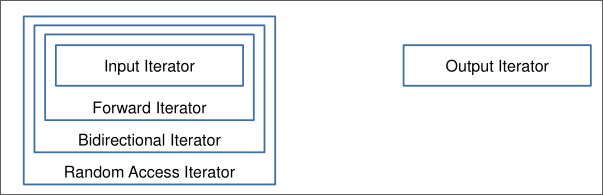
\includegraphics[scale=0.4]{2022-11-08-09_34_02.png}\newline
\textcolor{teal}{The more you move outwards on the input iterator, the more power these iterators have!}\\
\hline
Input Iterators & 
\begin{lstlisting}
struct input_iterator_tag{};
auto operator* () -> Element;
auto operator++() -> It&;
auto operator++(int) -> It;
auto operator==(It const&) -> bool;
auto operator!=(It const&) -> bool;
auto operator= (It const&) -> It&;
It(It const&); //copy ctor
\end{lstlisting} 
\, \newline
\begin{itemize}
\item \textcolor{orange}{Supports reading the "current" element}
\item \textcolor{orange}{Allows for one-pass input algorithms}\newline
  \textcolor{red}{Can't step backwards}
\item \textcolor{orange}{Models the std::istream\_iterator and std::istream}
\item \textcolor{orange}{Can be compared with == and !=}\newline
  To other iterator objects of teh sae type: It
\item \textcolor{orange}{Can be copied}\newline
  \textcolor{red}{After increment (calling ++) all other copies are invalid!}\newline
  *it++ is allowed explicitly (by the standard)
\vspace{-2mm}
\end{itemize}\\
\hline
\end{tabular}
\end{table}
\pagebreak
\begin{table}[ht!]
\begin{tabular}{|m{0.2\linewidth}|m{0.755\linewidth}|}
\hline
Forward Iterators &
\begin{lstlisting}
struct forward_iterator_tag{};
auto operator* () -> Element&;
auto operator++() -> It&;
auto operator++(int) -> It;
auto operator==(It const&) -> bool;
auto operator!=(It const&) -> bool;
auto operator= (It const&) -> It&;
It(It const&); //copy ctor
\end{lstlisting} 
\, \newline
\begin{itemize}
\item \textcolor{orange}{Can do whatever an input iterator can do, and:} \newline
  \textcolor{teal}{Supports changing the "current" element, unless elements are const}
\item \textcolor{orange}{Still allows only for one-pass input algorithms}\newline
  \textcolor{red}{Can't step backwards}\newline
  But can keep iterator copy around for later reference
\item \textcolor{orange}{Models the std::forward\_list iterators}
\vspace{-2mm}
\end{itemize} \\
\hline
Bidirectional Iterator & 
\begin{lstlisting}
struct bidirectional_iterator_tag{};
auto operator* () -> Element&;
auto operator++() -> It&;
auto operator++(int) -> It;
auto operator--() -> It&;
auto operator--(int) -> It;
auto operator==(It const&) -> bool;
auto operator!=(It const&) -> bool;
auto operator= (It const&) -> It&;
It(It const&); //copy ctor
\end{lstlisting}
\, \newline
\begin{itemize}
\item \textcolor{orange}{Can do whatever a forward iterator can, plus..}\newline
  \textcolor{red}{CAN GO BACKWARDS}
\item \textcolor{orange}{Allows for forward-backwards-pass algorithms}
\item \textcolor{orange}{Models the std::iterators}
\vspace{-2mm}
\end{itemize}\\ 
\hline
Random Access Iterators & 
\begin{lstlisting}
struct random_access_iterator_tag{};

auto operator* () -> Element&;
auto operator++() -> It&;
auto operator++(int) -> It;
auto operator--() -> It&;
auto operator--(int) -> It;
auto operator==(It const&) -> bool;
auto operator!=(It const&) -> bool;
auto operator= (It const&) -> It&;
It(It const&); //copy ctor
auto operator[](distance) -> Element&;
auto operator+(distance) -> It;
auto operator+=(distance) -> It&;
auto operator-(distance) -> It;
auto operator-=(distance) -> It&;
auto operator-(It const&) -> distance;
//relational operators, like <
\end{lstlisting}
\, \newline
\begin{itemize}
\item \textcolor{orange}{Can do whatever a bidirectional iterator can, plus..}\newline
  \begin{itemize}
  \item \textcolor{teal}{Directly access element at index (offset to current position): distance can be positive or negative}
  \item \textcolor{teal}{Go n steps forward or backwards}
  \item \textcolor{teal}{"Subtact" two iterators to get the distance}
  \item \textcolor{teal}{Compare with relational operators (<, <=, >, >=)}
  \end{itemize} 
\item \textcolor{orange}{Allows random access in algorithms}
\item \textcolor{orange}{Models the std::vector iterators}
\vspace{-2mm}
\end{itemize} \\
\hline
\end{tabular}
\end{table}
\pagebreak
\begin{table}[ht!]
\begin{tabular}{|m{0.2\linewidth}|m{0.755\linewidth}|}
\hline
Output Iterator & 
\begin{lstlisting}
struct output_iterator_tag{};
auto operator*() -> Element&;
auto operator++() -> It&;
auto operator++(int) -> It;
\end{lstlisting}
\, \newline
\begin{itemize}
\item \textcolor{orange}{Can write value to current element, but only once (*it = value)}\newline
  Then increment is required
\item \textcolor{orange}{Modeled after std::ostream\_iterator}
\item \textcolor{orange}{Most other iterators can also act as output iterators}\newline
  \textcolor{red}{Unless the underlying container is const}
\item \textcolor{orange}{Exception: associative containers will allow only read-only iteration}
\item \textcolor{orange}{No comparison and end to an out rang is not queryable}
\vspace{-2mm}
\end{itemize}\\ 
\hline
std::distance(start, goal) & 
\vspace{2mm}
\begin{itemize}
  \item \textcolor{orange}{counts the number of hops it needs to take to the goal}  
\item \textcolor{orange}{Efficient for random access iterators}
\item \textcolor{orange}{For other iterators it has to loop -> not efficient}\newline
  This also implies that the goal has to be after start.
\vspace{-2mm}
\end{itemize}\\ 
\hline
std::advance(itr, n) & 
\textcolor{orange}{std::advance simply moves x steps forward or backwards ( if the iterator allows it!)}\newline
\begin{itemize}
\item \textcolor{teal}{Efficient for random access iterators}
\item \textcolor{teal}{returns void -> no copies made}
\vspace{-2mm}
\end{itemize} \\
\hline
std::next() / std::prev() & 
\textcolor{orange}{Goes one step further/back on the iterator and returns a copy of the value in the container at the next index.}\newline
\textcolor{teal}{The step can be specified to be something other than 1 with a temporary argument!}\\
\hline
const iterators & 
\textcolor{red}{A const iterator does not mean that the iterator itself is const, only the elements behind it are! In other words, it just doesn't allow you to modify the elements behind it.}\newline
\begin{lstlisting}
std::vector v{3, 1, 4, 1, 5, 9, 2, 6};
auto const iter1 = values.begin(); //std::vector<int>::iterator const
++iter1;
auto iter2 = values.cbegin(); //std::vector<int>::const_iterator
*iter = 2;
\end{lstlisting}
\, \newline
\textcolor{teal}{Here we would try to change the value behind the iterator, this doesn't work with const iterators!}\\
\hline
\end{tabular}
\section{Algorithms}
\begin{tabular}{|m{0.2\linewidth}|m{0.755\linewidth}|}
\hline 
Different Algorithms and numberic functions & 
\textcolor{red}{All of these are defined in <algorithm>}\newline
\minipg{
Algorithms:\newline
\begin{itemize}
\item \textcolor{purple}{Filling}
\item \textcolor{purple}{Finding}
\item \textcolor{purple}{Property checking}
\item \textcolor{purple}{Transformation}
\end{itemize} 
}{
Numerics:\newline
\begin{itemize}
\item \textcolor{purple}{Generic numberic functions}
\item \textcolor{purple}{Some functions can be applied in on numeric contexts}
\end{itemize} 
}[0.4,0.4]\\
\hline
Why? & 
Why do we use algorithms over loops and other code?\newline
It is very simple, \textbf{algorithms are easy and safe to use without x amount of possibilities for errors!}\newline
Think about a loop, you need to make sure you are in the bounds of the vector, or that you assign the right value at each time...\newline
With algorithms we just say here is range go do stuff.
Reasons for algorithms:\newline
\begin{itemize}
\item \textcolor{purple}{Correctness}\newline
  Handwritten algorithms are often error prone and need time debugging!
\item \textcolor{purple}{Readability}\newline
  Handwritten algorithms are often conveluted and need lots of time reading and understanding.
\item \textcolor{purple}{Performance}\newline
  Unless you are very good at what you do, the standard algorithms are likely faster!
\vspace{-3mm}
\end{itemize} 
\\
\hline
for\_each & 
For loop using 2 iterators -> \textbf{begin()} and \textbf{end()} as well as a \textbf{lambda} as the function to execute on each element.\newline
\begin{lstlisting}
auto values = std::vector{3, 0, 1, 4, 0, 2};
auto f = [](auto v) {};
std::for_each(begin(values), end(values), f);
\end{lstlisting}\\
\hline
Functors & 
Functors are just overloaded structs or classes on the () operator.\newline
\textbf{As expected, you can then use this struct or class like it is a function!}\newline
Here is how to implement it:\newline 
\begin{lstlisting}
struct Accumulator {
  int accumulatedValue{0};
  auto operator()(int value) -> void {
    accumulatedValue += value;
  }
  int sum() const; // does what the function says above
};
auto sum(std::vector<int> values) -> int {
  Accumulator acc{};
  for(auto v : values) { acc(v); }
  return acc.sum();
}
 // OR
auto sum(std::vector<int> values) -> int {
  auto acc = Accumulator{};
  return std::for_each(begin(values), end(values), acc).sum();
}
\end{lstlisting}\\
\hline
\end{tabular}
\end{table}
\pagebreak
\begin{table}[ht!]
\begin{tabular}{|m{0.2\linewidth}|m{0.755\linewidth}|}
\hline
Additional Argument to Associative Containers & 
You can pass a bool lambda to associative containers, this means that the result of the predicate must be false or true.\newline
The idea is that you can give a sorting algorithm to the set in order to easily sort it out of the box.\newline
\begin{lstlisting}
std::set<int, std::greater<>> reverse_int_set{};
\end{lstlisting} 
\, \newline
\textcolor{OliveGreen}{Note that this lambda must be \textbf{transitive and irreflexive}}\newline
Transitive: \(x > y\) and \(y > z\), then also \(x > z\)\newline
Irreflexive: \\
\hline
Transform & 
Transform uses 2 vectors with a lambda to perform a function on each element in both vectors.\newline
\begin{lstlisting}
auto counts = std::vector{3, 0, 1, 4, 0, 2};
auto letters = std::vector{'g', 'a', 'u', 'y', 'f', 'o'};
auto combined = std::vector<std::string>{};
auto times = [](auto i, auto c) { return std::string(i, c); };
std::transform(begin(counts), end(counts), begin(letters),
std::back_inserter(combined), times);
\end{lstlisting}
\, \newline
Here we would print each character x amount of times, with x being the same index element in the counts vector.\\
\hline
Merge & 
Mergesort takes 2 sorted vectors and puts them together:\newline
\begin{lstlisting}
std::vector r1{9, 12, 17, 23, 54, 57, 85, 95};
std::vector r2{2, 30, 32, 41, 49, 63, 72, 88};
std::vector d(r1.size() + r2.size(), 0);
std::merge(begin(r1), end(r1), begin(r2), end(r2), begin(d));
// 2,9,12,17,23,30,32,41,49,54,57,63,72,85,88,95
\end{lstlisting}\\
\hline
Remove and Erase & 
\textcolor{red}{Remove will not actually \textbf{remove} the elements, instead, it will mark them as removable in order to not cause iterator invalidation!}\newline
\textcolor{OliveGreen}{If you want to properly remove them, then you can also call erase which will then free the marked elements!}\newline
\begin{lstlisting}
auto values = std::vector{54, 13, 17, 95, 2, 57, 12, 9};
auto is_prime = [](unsigned u) { u > 20};
auto removed = std::remove_if(begin(values), end(values), is_prime);
// mark 2,9,12,13,17 as to remove
values.erase(removed, values.end());
// erase the marked elements
// vector is now -> 54,57,95
\end{lstlisting} 
\, \newline
remove\_if just has an additional boolean check which can be done with a lambda, use case is shown here for filtering!\\
\hline
Accumulate & 
Sum function:\newline
\begin{lstlisting}
std::vector<std::string> longMonths{"Jan", "Mar", "May", "Jul", "Aug", "Oct", "Dec"};
auto accumulatedString = std::accumulate(
next(begin(longMonths)), //Second element
end(longMonths),
//End
longMonths.at(0),
//First element, usually the neutral element
[](std::string const& acc, std::string const& element) {
return acc + ", " + element;
}); //Jan, Mar, May, Jul, Aug, Oct, Dec
\end{lstlisting}\\
\hline
\_if suffix & 
Just like the remove\_if, there are many other algorithms that implement the if keyword to \textbf{only execute this algorithm when the boolean check is true}.\newline
Often they are used in combination with \textbf{lambdas}!
\begin{lstlisting}
auto numbers = std::set{1, 2, 3, 4, 5, 6, 7, 8, 9};
auto isPrime = [](auto u) {/*...*/};
auto nOfPrimes = std::count_if(begin(numbers), end(numbers), isPrime);
\end{lstlisting}
\, \newline
List of Algorithms with the if suffix:\newline
\minipg{
\begin{itemize}
\item \textcolor{teal}{count\_if}
\item \textcolor{teal}{find\_if}
\item \textcolor{teal}{find\_if\_not}
\item \textcolor{teal}{copy\_if}
\end{itemize} 
}{\begin{itemize}
\item \textcolor{teal}{count\_if}
\item \textcolor{teal}{find\_if}
\item \textcolor{teal}{find\_if\_not}
\item \textcolor{teal}{copy\_if}
\end{itemize} 
}[0.4,0.4]\\
\hline
Algorithms \_n Versions & 
Instead of always going through the entire list, you can also use the \_n suffix algorithms to specify a different endpoint for this algorithm, for example in a vector with 7 elements you might want to only do the first 5 elements, therefore the additional parameter will be 5, for 5 elements!\newline
\begin{lstlisting}
auto numbers = std::set{1, 2, 3, 4, 5, 6, 7, 8, 9};
auto top5 = std::vector<int>(5);
std::copy_n(rbegin(numbers), 5, begin(top5));
\end{lstlisting}
\, \newline
\begin{itemize}
\item \textcolor{teal}{search\_n}
\item \textcolor{teal}{copy\_n}
\item \textcolor{teal}{fill\_n}
\item \textcolor{teal}{generate\_n}
\item \textcolor{teal}{for\_each\_n}
\vspace{-3mm}
\end{itemize}\\ 
\hline
Heap Algorithm & 
\begin{lstlisting}
std::vector<int> v{3,1,4,1,5,9,2,6};
make_heap(v.begin(),v.end());
pop_heap(v.begin(),v.end());
v.pop_back();
v.push_back(8);
push_heap(v.begin(),v.end());
sort_heap(v.begin(),v.end());
\end{lstlisting}\\
\hline
\end{tabular}
\end{table}
\pagebreak
\begin{table}[ht!]
\begin{tabular}{|m{0.2\linewidth}|m{0.755\linewidth}|}
\hline
Don't mixmatch Iterators & 
\textcolor{red}{Don't mixmatch iterators!}:\newline
\begin{lstlisting}
std::vector<unsigned> values1 = create_vector();
std::vector<unsigned> values2 = create_vector();
auto f = [](unsigned u) {/*...*/};
std::for_each(begin(values1), end(values2), f);
\end{lstlisting}
\\
\hline
Make sure that enough space is allocated in a vector & 
\textcolor{red}{Make sure that enough space is allocated for when you copy data!}\newline
\begin{lstlisting}
std::set<unsigned> numbers{1, 2, 3, 4, 5, 6, 7, 8, 9};
std::vector<unsigned> primes{};
auto isPrime = [](unsigned u) {/*...*/};
std::copy_if(begin(numbers), end(numbers), begin(primes), isPrime);
\end{lstlisting}
\, \newline
So how do we properly do this? \textbf{Inserters!}\newline
\begin{lstlisting}
std::set<unsigned> numbers{1, 2, 3, 4, 5, 6, 7, 8, 9};
std::vector<unsigned> primes{};
auto is_prime = [](unsigned u) {/*...*/};
std::copy_if(begin(numbers), end(numbers), back_inserter(primes), is_prime);
\end{lstlisting}
\, \newline
There are 3 such inserters:\newline
\begin{itemize}
\item \textcolor{purple}{back\_inserter}\newline
  uses the \textbf{push\_back function} to insert at the back
\item \textcolor{purple}{front\_inserter}\newline
  uses the \textbf{push\_front function} to insert at the front
\item \textcolor{purple}{inserter}\newline
  uses the \textbf{insert member} function to insert
\item \textcolor{purple}{item 4}
\vspace{-3mm}
\end{itemize} \\
\hline
Iterator invalidation & 
If you change a vectors size during an algorithm or a loop, you have the problem that your vector might change size. \newline
The side effect is that \textbf{your vector will resize!} This means that \textbf{it will move to another memory location!}\newline
Because of the new memory location \textbf{your iterators are now invalid!}\newline
Avoid modifying vector sizes during iteration, instead use the same system as the remove does, mark them and then modify the vector size later or create a new one.\\
\hline
Using ranges & 
You can of course also use ranges instead should they work with your compiler, lol :P\newline
\begin{lstlisting}
auto values = std::vector<int>{3, 1, 4, 1, 5, 9};
// old
std::reverse(begin(values), end(values));
// new
std::ranges::reverse(values);
\end{lstlisting}\\
\hline
Non-Modifying Algorithms & 
\vspace{2mm}
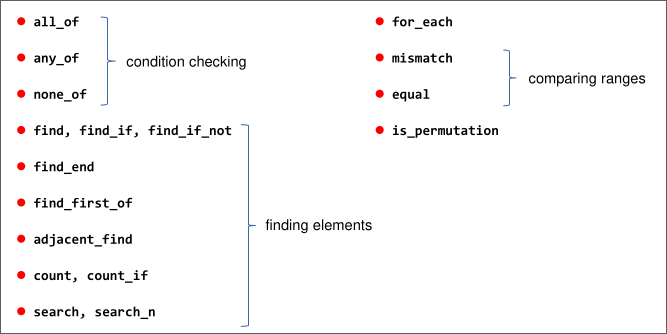
\includegraphics[scale=0.4]{2022-11-15-09_43_09.png}\\
\hline
Mutating Sequence Operations & 
\vspace{2mm}
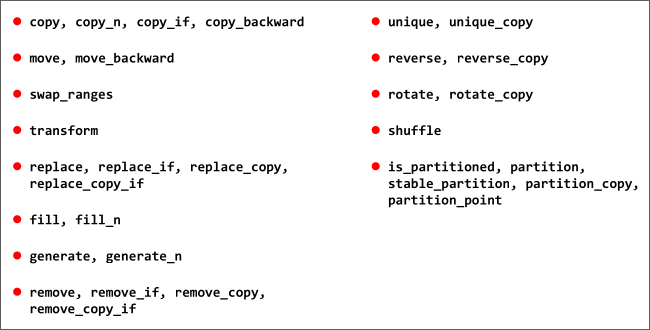
\includegraphics[scale=0.4]{2022-11-15-09_43_15.png}\\
\hline
Sorting Algorithms and Related Operations & 
\vspace{2mm}
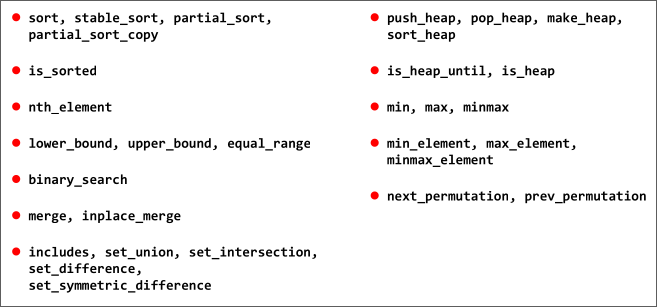
\includegraphics[scale=0.4]{2022-11-15-09_43_22.png}\\
\hline
\end{tabular}
\end{table}
\pagebreak
\begin{table}[ht!]
\section{Templates}
\begin{tabular}{|m{0.2\linewidth}|m{0.755\linewidth}|}
\hline
Basics & 
You can use one or more types to use in templates.\newline
\textcolor{OliveGreen}{Note that you usually write the template definition inside the header file!\newline
\textbf{This also means that templates are implicitly inline!!}}\newline
\begin{lstlisting}
template <typename T>
  auto min(T left, T right) -> T {
    return left < right ? left : right;
}
\end{lstlisting}
\, \newline
For the writing in the header file part, the reason for this is that you could only use that template function inside of one cpp file. Usually this makes no sense so we define it in the header, this way we can export the function.\\
\hline
Compiler checks & 
The compiler checks the template code twice, the first time when it sees the template function itself, here it only does basic syntax checking, does the template make sense, are there any missing semicolons etc.\newline
The next time it checks is at instantiation, here it will do proper checking, like can this type actually be used in this function with all the operators that are used here?\\
\hline
Duck typing & 
"If it walks and quacks like a duck, it must be a duck"\newline
C++ has a similar way of doing generics as rust, it will simply do the operation if the type has said operation.\newline
In rust the same is guaranteed, the only difference is that the guarantee usually comes from a trait, while in c++ it must come from the type itself.\newline
With c++ 20 you can technically also do the same in c++ as you did in rust, but once again funny funny maybe worky maybe noty.\\
\hline
Type matching & 
The c++ compiler only does extremely exact matching, meaning a double and an int will not match to either double double or int int:\newline
\minipg{
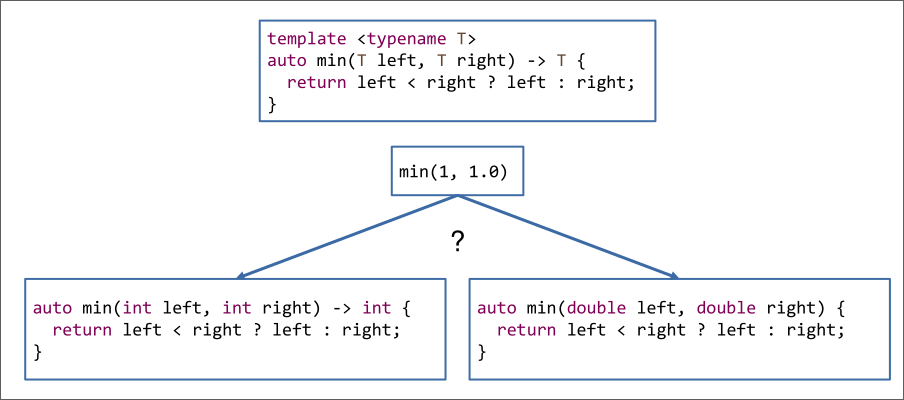
\includegraphics[scale=0.3]{2022-11-22-08_46_33.png}
}{
\textcolor{red}{ERROR BRO}
}[0.5,0.25]\\
\hline
Variable templates & 
C++ compiler allows for a variable number of templates which can then also be used in a function!\newline
\begin{lstlisting}
auto printAll() -> void {} // needed for printAll with the last case where first is empty!
template<typename First, typename...Types>
  auto printAll(First const& first, Types const&...rest) -> void {
  std::cout << first;
  if (sizeof...(Types)) {
    std::cout << ", ";
  }
  printAll(rest...); // print the variable numbers of parameters
}
\end{lstlisting}
\, \newline
\textcolor{OliveGreen}{Note that the variable number of types needs to be the last part of both the template and the parameter list!!}\\
\hline
Packing and unpacking & 
As you can see above and similar to rust, you can use the ... operator to indicate packing inside the template functions.\newline
Here it will put together the types with \textbf{Types const \&...rest} and then unpack to use again inside a function with \textbf{rest...}\newline
\textcolor{OliveGreen}{This is just syntax sugar, the code that will be generated will have hardcoded variables again, you just don't see them in c++ -> only in machine code!}\\
\hline
Template overloading & 
You can overload a template if you for example want to use pointers instead of the actual type, or you can even write an overload for an explicit type:\newline
\begin{lstlisting}
template <typename T> // regular types
  auto min(T left, T right) -> T {
    return left < right ? left : right;
}
template <typename T> // specific to pointers
  auto* min(T* left, T* right) -> T {
    return *left < *right ? left : right;
}
auto min(char const* left, char const* right) -> char const* {
  return std::string{left} < std::string{right} ? left : right;
} // overload for explicit type
\end{lstlisting}\\
\hline
Generic Operator functions &
You can create generic operator functions with either a struct or a lambda, but this might not always work, as there are often more specific matches which will be called instead!\newline
\begin{lstlisting}
// lambda
auto const printer = [&out](auto const& e) {
  out << "Element: " << e;
};
// struct method
struct __PrinterLambda {
  template <typename T>
  auto operator()(T const& e) const -> void {
    __out << "Element: " << e;
  }
  std::ostream & __out;
};
\end{lstlisting}\\
\hline
\end{tabular}
\end{table}
\pagebreak
\begin{table}[ht!]
\begin{tabular}{|m{0.2\linewidth}|m{0.755\linewidth}|}
\hline
Converting C string literals to c++ standard literals & 
C string literals are stored in a char array, this makes it hard to be used, as arrays don't have any special functions attached to them.\newline
We can instead use std::string\_literals to for example make printing work with string literals:\newline
\begin{lstlisting}
using namespace std::string_literals;
std::cout << min("C++"s, "Java"s);
\end{lstlisting}\\
\hline
More specificity problems & 
\begin{lstlisting}
template <typename T>
  auto min(T& left, T& right) -> T {
    return left < right ? left : right;
}
auto min(std::string const& left, std::string const& right) -> std::string {
  return std::ranges::lexicographical_compare(left, right, [](char l, char r) {
    return tolower(l) < tolower(r);
  }) ? left : right;
}
std::string small{"aa"};
std::string capital{"ZZ"};
std::cout << min(small, capital) << '\n'; //ZZ
\end{lstlisting} 
\, \newline
Here the problem would be that we didn't specify the string as const, this mean the template would be called, which didn't specify that we want to compare the lower symbols only. Bigger symbols are always higher up in the ascii table, meaning we get the wrong behavior with ZZ being "smaller" than aa!\\
\hline
Dangling references or rather why to use rust & 
The following is exactly why borrowing just works, we pass 2 references to a function and receive the value of one of them. The problem is that the lifetime of the temporary reference of the parameters will be invalid after the semicolon, exactly like in rust!\newline
This means you could potentially be getting invalid values!\newline 
\begin{lstlisting}
template <typename T>
auto const& min(T const& left, T const& right) -> T {
return left < right ? left : right;
// left and right now dead as lifetime not extended
// in other words, return is invalid
}
std::string const& smaller = min("a"s, "b"s);
std::cout << "smaller is: " << smaller; // undefined behavior! might or might not work!
\end{lstlisting}
\, \newline
\textcolor{OliveGreen}{The fix is to return a const \& reference as well, as this would extend the lifetime of the reference!}\newline
\begin{lstlisting}
template <typename T>
auto min(T const& left, T const& right) -> T const& {
  return left < right ? left : right;
}
\end{lstlisting}\\
\hline
\end{tabular}
\section{Class Templates}
\begin{tabular}{|m{0.2\linewidth}|m{0.755\linewidth}|}
\hline
Basics & 
These are the same as before, just nested within a class to give you flexiblity to create a generic class. \newline
\begin{lstlisting}
template <typename T> class Sack {
  using SackType = std::vector<T>;
  // ATTENTION, typename needed here for size_type.
  using size_type = typename SackType::size_type;
  SackType theSack{};
public:
  auto empty() const -> bool {
    return theSack.empty();
  }
  auto size() const -> size_type{
    return theSack.size();
  }
  auto putInto(T const& item) -> void {
    theSack.push_back(item);
  }
  auto getOut() -> T; //Implementation out of line
};
\end{lstlisting}\\
\hline
Typedef vs using & 
Use using instead of typedef as it is newer and can do the following while typedef can't:\newline
\begin{lstlisting}
// ok
using someName = std::vector<T>;
// ERROR BRO
typedef std::vector<T> someName;
\end{lstlisting}\\
\hline
Typename for dependent names & 
Within the template definition you might use names that are directly or indirectly depending on the template parameter.\newline
This would mean an endless loop of dependency, to solve this we need to use typename.\newline
\begin{lstlisting}
// examples
template <typename T> void accessTsMembers() {
  typename T::MemberType m{};
  T::StaticMemberFunction();
  T::StaticMemberVariable;
}

template<typename T> class Sack {
  using size_type = typename std::vector<T>::size_type;
  //...
};
\end{lstlisting}\\
\hline
\end{tabular}
\end{table}
\pagebreak 
\begin{table}[ht!]
\begin{tabular}{|m{0.2\linewidth}|m{0.755\linewidth}|}
\hline
Static Member variables &
Static Member variables are \textbf{semi global variables with a double colon scope.}\newline
\textcolor{purple}{Global in the sense of each individual type has their own version of it. So if we override the variant for integers, then each integer will access the same value!}\newline
You can add static structs via inline like this: \newline
\begin{lstlisting}
template <typename T> struct StaticMember {
  inline static int member{sizeof(T)};
};
\end{lstlisting}
\, \newline
Here an example how you can use this: \newline
\begin{lstlisting}
// class.hpp
template <typename T> struct StaticMember {
  inline static int member{sizeof(T)};
};

// class.cpp
#include "staticMember.hpp"
auto setMemberTo42() -> int {
  using MemberType = StaticMember<int>;
  MemberType::member = 42;
  return MemberType::member;
}

// main.cpp
#include "staticMember.hpp"
#include <iostream>
auto setMemberTo42() -> int;
auto main() -> int {
  std::cout << StaticMember<double>::member << '\n'; // 8
  std::cout << StaticMember<int>::member << '\n';    // 4
  std::cout << setMemberTo42() << '\n'; // overrides!   42
  std::cout << StaticMember<int>::member << '\n';    // 42
}
\end{lstlisting}\\
\hline
Dependent names and specificity in template classes & 
For templates it is better to use the this keyword as otherwise you could potentially use another function that is not inside the class.\newline
To avoid this, you can add either double colons or the this keyword to avoid problems.\newline 
\begin{lstlisting}
template <typename T>
struct Parent {
  auto foo() const -> int { // can be called with this->foo()
  return 42;
  }
  static int const bar{43}; // accessed with this->bar
};
auto foo() -> int { // can be called with foo()
  return 1;
}
double const bar{3.14}; // accessed with bar
\end{lstlisting}\\
\hline
Containers with pointers & 
When we use pointers in containers, we have the problem that we can create containers with pointers inside them. \newline
As expected nobody will give us the guarantee that these pointers will still be valid at any given time.\newline
To solve this we can create a specific template that is more specific to pointer which makes sure we will not have this issue:\newline
\begin{lstlisting}
// Partial Specialization
template <typename T>
struct Sack<T *>;

// Explicit Specialization
template <>
struct Sack<char const *>;
\end{lstlisting} 
\, \newline
These can then be used to make sure that the values will still be valid.\newline
We can however, also just prevent the creation of point based containers:\newline
\begin{lstlisting}
template <typename T> struct Sack<T *> {
  ~Sack() = delete; // lmao delete constructor
};

// while the char const can be done with something like std::vector<string> instead
template <> struct Sack<char const *> {
  using SackType = std::vector<std::string>;
  using size_type = SackType::size_type;
  SackType theSack;
}
\end{lstlisting}\\
\hline
Type casting overload & 
In order to cast a type to another, you must overload the operator for this, or use another function instead:\newline
\begin{lstlisting}
// Overload 
template <typename Elt>
  explicit operator std::vector<Elt>() const {
    return std::vector<Elt>(begin(theSack), end(theSack));
}

// other function 
template <typename Elt = T>
  auto asVector() const {
  return std::vector<Elt>(begin(theSack), end(theSack));
}
\end{lstlisting}\\
\hline
\end{tabular}
\end{table}
\pagebreak 
\begin{table}[ht!]
\begin{tabular}{|m{0.2\linewidth}|m{0.755\linewidth}|}
\hline
Type deduction with structs & 
Since C++ 17 the compiler can deduce the typename that you have specified at the top when using functions from classes etc: \newline
\begin{lstlisting}
template <typename T> struct Box {
  Box(T content) : content{content}{}
  T content;
};
auto main() -> int {
  Box<int> b0{0}; //Before C++17
  Box      b1{1}; //Since C++17
}
\end{lstlisting} \\
\hline
Type deduction with initializer lists & 
Initializer list allow us to create a container without specifiying the type, as it is implicitly passed by the values that you enter:\newline
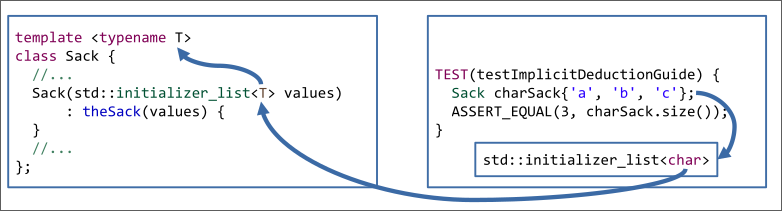
\includegraphics[scale=0.4]{2022-11-29-09_27_18.png}\\
\hline
Type deduction with Iterators & 
When we want to use type deduction with iterators, then we need a way to do this with iterators.\newline
Obviously this is not done out of the box, therefore we need another way to do this: \newline
\begin{lstlisting}
template <typename Iter>
Sack(Iter begin, Iter end) -> Sack<typename std::iterator_traits<Iter>::value_type>;

TEST(testDeductionForIterators) {
  std::vector values{3, 1, 4, 1, 5, 9, 2, 6};
  Sack aSack(begin(values), end(values));
  ASSERT_EQUAL(values.size(), aSack.size());
}
// Note without the template above, aSack would not compile!
\end{lstlisting}\\
\hline
Passing a standard container as template parameter & 
Sometimes we want to have a container itself as a template container, which will be used instead of one harcoded variant.\newline
\begin{lstlisting}
Sack<unsigned, std::set> aSack{1, 2, 3};

auto getOut() -> T {
  throwIfEmpty();
  auto index = static_cast<size_type>(rand() % size());
  auto it = begin(theSack);
  advance(it, index);
  T retval{*it};
  theSack.erase(it);
  return retval;
}
\end{lstlisting}\\
\hline
Variadic Templates & 
Normally we have a set of parameters that a template wants, eg. types,containers etc. This means that we can't use initializer lists when passing a container to another container as a template parameter, unless, you use \textbf{variadic template}:\newline
\begin{lstlisting}
// Note the end is the default value, include this to make sure defualt constructors will still work!!
template <typename T, template<typename...> typename Container = std::vector>
class Sack;

Sack<unsigned, std::set> aSack{1, 2, 3}; //Works
\end{lstlisting}\\
\hline
Non-type parameters & 
You can also specify non-type parameters for things like size of arrays etc:\newline
\begin{lstlisting}
template <typename T, std::size_t n>
  auto average(std::array<T, n> const& values) {
  auto sumOfValues = accumulate(begin(values), end(values), 0);
  return sumOfValues / n;
}

// You can also use auto if the non-type parameter should be flexible
template <typename T, auto n>
  auto average(std::array<T, n> const& values) {
  auto sumOfValues = accumulate(begin(values), end(values), 0);
  return sumOfValues / n;
}
\end{lstlisting}\\
\hline
\end{tabular}
\end{table}
\pagebreak
\begin{table}[ht!]
\begin{tabular}{|m{0.2\linewidth}|m{0.755\linewidth}|}
\hline
\end{tabular}
\end{table}
\pagebreak
\begin{table}[ht!]
\section{Pointers and Heap}
\begin{tabular}{|m{0.2\linewidth}|m{0.755\linewidth}|}
\hline
When to use Heap & 
\vspace{2mm}
\begin{itemize}
\item \textcolor{purple}{Stack memory isn't sufficient}
\item \textcolor{purple}{Scope/lifetime is dynamic/unclear}
\end{itemize} 
\, \newline
Note however, that you should generally try to use stack over heap, for both \textbf{performance and memory security!}\newline
\textcolor{orange}{Generally rely on constructor and destructor!}\\
\hline
Legacy & 
Eh yeah, don't, hehe, me use raw pointer, me monke:\newline
\begin{lstlisting}
auto ptr = new int{};
std::cout << *ptr << '\n';
delete ptr;
\end{lstlisting} 
\, \newline
Note, not using free leads to \textbf{memory leak}, while \textbf{double freeing leads to other undefined behavior}.\\
\hline
std::unique\_ptr & 
\vspace{2mm}
\begin{itemize}
\item \textcolor{purple}{Single Owner}
\item \textcolor{purple}{Can wrap C style pointers to interact with legacy code}
\item \textcolor{purple}{Not "best" for class hierarchies -> multiple parent not possible due to single owner}\newline
  \textcolor{orange}{Use shared pointer instead}
\item \textcolor{purple}{Can't be copied due to single owner!}
\item \textcolor{purple}{Memory freed when out of scope -> like rust}
\item \textcolor{purple}{Only compile overhead!}
\end{itemize} 
\begin{lstlisting}
auto factory(int i) -> std::unique_ptr<X> {
  return std::make_unique<X>(i);
}
// or only local!
std::unique_ptr<T> ptr = std::make_unique<T>(); // local
\end{lstlisting}
\\
\hline
std::shared\_ptr & 
This sounds like Ref<A> from rust, but unlike rust, you can have \textbf{multiple MUTABLE pointers!}\newline
This means that you can get into trouble with concurrency!\newline
\textcolor{purple}{will be alive until the last shared\_pointer goes out of scope.}\newline
\textcolor{purple}{This is more memory intensive than unique\_pointers, as it needs to store more information -> reference count etc}\newline
\begin{lstlisting}
struct A {
  A(int a, std::string b, char c);
};
auto createA() -> std::shared_ptr<A> {
  return std::make_shared<A>(5, "hi", 'a');
}
auto main() -> int {
  auto anA = createA();
  auto sameA = anA; //second pointer to same object
  A copyA{*sameA}; //copy ctor.
  auto another = std::make_shared<A>(copyA); //copy ctor on heap
}
\end{lstlisting}
\\
\hline
std::move() & 
This is the same as move in rust, it takes the value and pushes it into another pointer.\newline
In other words, it invalidates one pointer and assigns a new pointer to the memory address.\newline
\begin{lstlisting}
#include <iostream>
#include <memory>
#include <utility>

auto create(int i) -> std::unique_ptr<int> {
  return std::make_unique<int>(i);
}
auto main() -> int {
  auto pi = create(42); // pointer pi to address of 42
  auto pj = std::move(pi); // 42 moved to pj
}
\end{lstlisting}
\\
\hline
Cyclic Issues & 
Just like with Ref<A>, shared pointers can have cyclic references that reference each other, therefore not deleting the objects as probably intended!\newline
\begin{lstlisting}
using HalfElfPtr = std::shared_ptr<struct HalfElf>;
struct HalfElf {
  explicit HalfElf(std::string name) : name{name}{}
  std::string name{};
  std::vector<HalfElfPtr> siblings{};
};
void middleEarth() {
  auto elrond = std::make_shared<HalfElf>("Elrond");
  auto elros = std::make_shared<HalfElf>("Elros");
  elrond->siblings.push_back(elros); // ref count 2
  elros->siblings.push_back(elrond); // ref count 2 
  // oops, they now point at each other, therefore it will never be deleted!
}
\end{lstlisting}\\
\hline
\end{tabular}
\end{table}
\pagebreak
\begin{table}[ht!]
\begin{tabular}{|m{0.2\linewidth}|m{0.755\linewidth}|}
\hline
std::weak\_ptr & 
Just like in rust we also have a weak pointer that will not keep an object alive, instead it is just counted up and down, and can be casted to a proper pointer when needed:\newline
\textcolor{orange}{Just like in rust, weak pointers are ignored when deleting! This means the object will be deleted despite weak pointers being available, making parent-child cascade deletion possible!}\newline
\begin{lstlisting}
struct Person {
  std::shared_ptr<Person> child;
  std::weak_ptr<Person> parent;

  auto Person::acquireMoney() const -> void {
  auto locked = parent.lock(); // try to aquire shared_pointer
    if (locked) { // parent is alive
      begForMoney(*locked);
    } else { // not aquired, pointer invalid
      goToTheBank();
    }
  }
};
\end{lstlisting} \\
\hline
& 
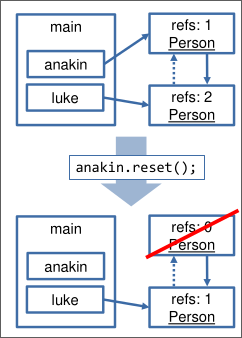
\includegraphics[scale=0.4]{2022-12-06-09_31_47.png}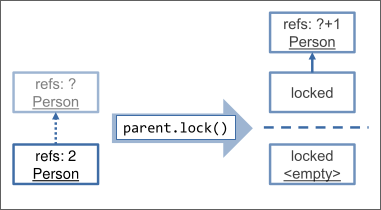
\includegraphics[scale=0.4]{2022-12-06-09_31_52.png}\\
\hline
Curiously Recurring Template Pattern (CRTP) & 
This is used when you want parents to be able to spawn their own children, in other words giving us a \textbf{weak pointer to ourselves}:\newline
\begin{lstlisting}
struct Person : std::enable_shared_from_this<Person> {
  std::shared_ptr<Person> child;
  std::weak_ptr<Person> parent;

  auto spawn() -> std::shared_ptr<Person> {
    child = std::make_shared<Person>();
    child->parent = weak_from_this(); // get new weak
    return child;
  }
};
\end{lstlisting} 
\, \newline
\textcolor{red}{Note, that this is only possible, if the parent \textbf{was created with a shared pointer!}}\\
\hline
Unique Pointer Interaction with C code & 
\vspace{2mm}
\begin{lstlisting}
struct free_deleter {
  template<typename T>
  auto operator()(T * p) const -> void {
    free(const_cast<std::remove_const_t<T> *>(p));
  }
};
template<typename T>
  using unique_C_ptr = std::unique_ptr<T, free_deleter>;
auto plain_demangle(char const * name) -> std::string {
  unique_C_ptr<char> toBeFreed{__cxxabiv1::__cxa_demangle(name, 0, 0, 0)};
  std::string result(toBeFreed.get());
  return result;
}
\end{lstlisting}\\
\hline
Storing smart pointers in vectors & 
\vspace{2mm}
\begin{lstlisting}
using PersonPtr = std::shared_ptr<struct Person>;
struct Person {
private:
  std::vector<PersonPtr> children;
  std::weak_ptr<Person> mother;
  std::weak_ptr<Person> father;
};
\end{lstlisting}\\
\hline
General & 
\vspace{2mm}
\begin{itemize}
\item \textcolor{purple}{Avoid using raw pointers}
\item \textcolor{purple}{Use stack whenever possible}
\item \textcolor{purple}{Avoid circular objects like linked lists etc when handling things with shared\_pointer}
\item \textcolor{purple}{Copying/Destroying is slow with shared\_pointer due to atomic counter}
\vspace{-3mm}
\end{itemize}\\ 
\hline
\end{tabular}
\end{table}
\pagebreak
\begin{table}[ht!]
\section{Dynamic Polymorphism}
\begin{tabular}{|m{0.2\linewidth}|m{0.755\linewidth}|}
\hline
Multi Inheritance & 
In c++, you can inherit from multiple classes, the order in which is inherited is based on the order that we specify the inheritance on.\newline
\begin{lstlisting}
class Base {};
struct MixIn {};
struct MultipleBases : public Base, private MixIn {};
\end{lstlisting}
\, \newline
\textcolor{red}{Note that in order to use pointers and interface like usecases, you need to import public, as private makes EVERYTING private, while public will keep the classification of the parent!}\\
\hline
Initializer List of parents & 
\vspace{2mm}
\begin{lstlisting}
class DerivedWithCtor : public Base1, public Base2 {
  int mvar;
public:
  DerivedWithCtor(int i, int j) :
  Base1{i}, Base2{}, mvar{j} {}
};
\end{lstlisting}
\, \newline
Parent Constructor can be called in the initializer list of a child class, note that \textbf{the order does not matter here, it only matters in the specification of inheritance at the top.}\\
\hline
Constructor Order & 
\textcolor{red}{The first constructor that will be called is the child constructor, this means that its elements will also be created first!}\newline
For example, because of the child being created first, this following program has undefined behavior, as \textbf{mvar is not initialized!}\newline
\begin{lstlisting}
struct Base1 {
  explicit Base1(int value) {
    std::cout << "Base1 with argument " << value << "\n";
  }
};
struct Base2 {
  Base2() { std::cout << "Base2\n"; }
};
class DerivedWithCtor : public Base1, public Base2 {
  int mvar;
public:
  DerivedWithCtor(int i, int j)
  : mvar{j}, Base2{}, Base1{mvar} {}
};
auto main() -> int {
  DerivedWithCtor dwc{1, 2};
}
\end{lstlisting}
\\
\hline
Behavior & 
\vspace{2mm}
\begin{itemize}
\item \textcolor{orange}{Operator overloading and function overloading allow polymorphic behavior at compile time }
\item \textcolor{orange}{Dynamic polymorphism needs obect references or smart pointers to work}\newline
  \begin{itemize}
  \item \textcolor{black}{Syntax overhead}
  \item \textcolor{black}{The base interface must be a good abstraction}
  \item \textcolor{black}{Copying carries the danger of \textbf{slicing -> only partial copy}}
  \end{itemize} 
\item \textcolor{orange}{Allow us more flexibility at run-time}\newline
  choose concrete implementation at run-time -> can give us more performance
\item \textcolor{orange}{If run-time flexibility is not needed, then templates are likely the better choice!}
\vspace{-3mm}
\end{itemize} 
\\
\hline
Shadowing &
When both the parent and the child implement the same function or variable, then the distinction on what will be called is the \textbf{Type}, this means that when a function take a parent class as parameter, then the parent function will be called, while the child function will be called should the function take the child as a parameter.\newline
\begin{lstlisting}
struct Base {
  auto sayHello() const -> void {
    std::cout << "Hi, I'm Base\n";
  }
};
struct Derived : Base {
  auto sayHello() const -> void {
    std::cout << "Hi, I'm Derived\n";
  } // redefinition of sayHello, will be used instead of parent function
};
\end{lstlisting}
\\
\hline
Overriding Parent functions & 
In order to avoid shadowing, we need to define the parent function as \textbf{virtual}, this makes it clear, that children might override this function!\newline
\begin{lstlisting}
struct Base {
  virtual auto sayHello() const -> void {
    std::cout << "Hi, I'm Base\n";
  }
};
struct Derived : Base {
  virtual auto sayHello() const override -> void {
    std::cout << "Hi, I'm Derived\n";
  } 
};
\end{lstlisting}
\, \newline
\textcolor{red}{note the override is optional, but just do it as it prevents shadowing!!!}\newline
Also note that when using override, the signature of the functions need to be identical! In other words, unlike with overloading, parameters and return types need to be the same!\newline
\textcolor{purple}{Also, if the \textbf{base class function is virtual, then EVERY iteration of this function, no matter how many inheritances, they are ALL implicitly virtual!!}}
\\
\hline
\end{tabular}
\end{table}
\pagebreak
\begin{table}[ht!]
\begin{tabular}{|m{0.2\linewidth}|m{0.755\linewidth}|}
\hline
Reference vs Value with polymorphism & 
\textcolor{red}{Important, the entire "we check what function will be called", can only be done dynamically, if the parameter is a reference!}\newline
\begin{lstlisting}
// value always uses the type
auto greet(Base base) -> void {
  //always calls Base::sayHello
  base.sayHello();
}
// reference takes the resolved type -> here child class
auto greet(Base const& base) -> void {
  //calls sayHello() of the actual type
  base.sayHello();
}
\end{lstlisting} 
\, \newline
\textcolor{purple}{Obviously, dynamic type resolution also happens with pointers, both smart and "dumb".}\\
\hline
Pure Virtual Functions & 
Pure virtual functions are abstract functions that are essentially not implemented.\newline
This also means that anyone who inherits from this class needs to implement this function!\newline 
\begin{lstlisting}
struct AbstractBase {
  virtual void doitnow() = 0;
};
AbstractBase create() {
  return AbstractBase{};
}
\end{lstlisting}
\, \newline
\textcolor{purple}{Note, as soon as you create even 1 pure virtual function, you can no longer instantiate the class that has such a pure virtual function!}\\
\hline
Virtual Destructor & 
Because things like unique pointer are extremely optimized, you need to define destructors as virtual if you want the actual resolved type to call it's destructor, otherwise all the extra mememory of the child class is ignored!!\newline
Small hint, the same would apply to new and delete.\newline
\begin{lstlisting}
struct Fuel {
  virtual auto burn() -> void = 0;
  virtual ~Fuel() { std::cout << "put into trash\n"; }
};
struct Plutonium : Fuel {
  auto burn() -> void { std::cout << "split core\n"; }
  ~Plutonium() { std::cout << "store many years\n"; }
};
auto main() -> int {
  std::unique_ptr<Fuel> surprise = std::make_unique<Plutonium>();
}
\end{lstlisting} 
\, \newline
\textcolor{purple}{The shared pointer would store the underlying type and do it correctly either way, but as said just write it, this makes it work with everything!}\\
\hline
General advice & 
\vspace{2mm}
\begin{itemize}
\item \textcolor{purple}{Use OOP sparingly, meaning that not everything should always inherit from everything!}
\item \textcolor{purple}{Often inheritance concepts do not work for everything}\newline
  all birds have the function fly, but what about penguins?
\item \textcolor{purple}{Changes in Base class need to be reverberated in every childclass}
\item \textcolor{purple}{Interaction between different hierarchies can be painful}
\vspace{-3mm}
\end{itemize} 
\\
\hline
Problems with copy constructor & 
We have already noted, that sometimes we copy not the entire object, but part of it, something like this happens when trying to copy references:\newline
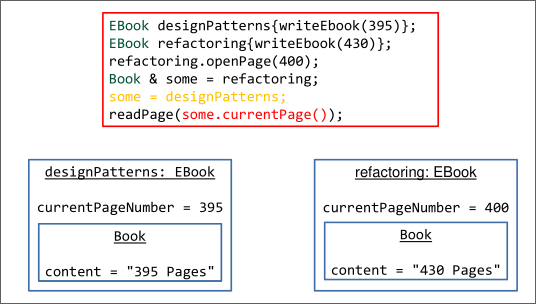
\includegraphics[scale=0.3]{2022-12-13-09_44_45.png}\newline
The easiest solution here is to simply delete the copy constructor, this prevents shallow copying a reference into another.\newline
\begin{lstlisting}
struct Book {
  //...
  auto operator=(Book const& other) -> Book & = delete;
  Book(Book const& other) = delete;
};
struct EBook : Book {
  // or simply manually override the copy constructor
  EBook(EBook const& other) :
  Book{pages},
  currentPageNumber{other.currentPageNumber}{}
  auto operator=(EBook const& other) -> EBook & {
    pages = other.pages;
    currentPageNumber = other.currentPageNumber;
    return *this;
  }
};
\end{lstlisting}
\\
\hline
\end{tabular}
\end{table}
\pagebreak
\begin{table}[ht!]
\begin{tabular}{|m{0.2\linewidth}|m{0.755\linewidth}|}
\hline
Using in classes to prevent hiding & 
You can prevent hiding with a \textbf{using} statement.\newline
This means that you would use the original function of the base class alongside the new one.\newline
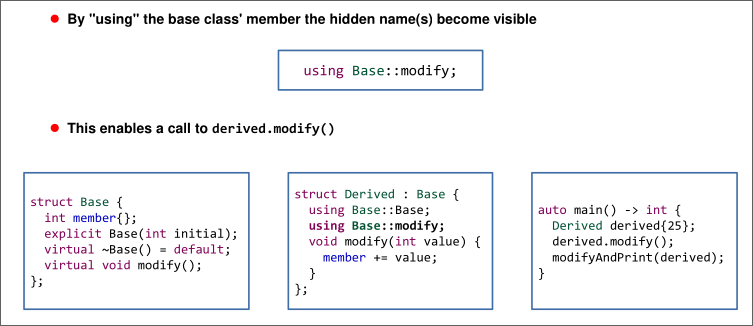
\includegraphics[scale=0.4]{2022-12-13-12_08_35.png}\\
\hline
\end{tabular}
\section{Initialization}
\begin{tabular}{|m{0.2\linewidth}|m{0.755\linewidth}|}
\hline
Types of Initialization & 
\vspace{2mm}
\begin{itemize}
\item \textcolor{purple}{Default Initialization}
\item \textcolor{purple}{Value Initialization}
\item \textcolor{purple}{Direct Initialization}
\item \textcolor{purple}{Copy Initialization}
\item \textcolor{purple}{List Initialization}
\item \textcolor{purple}{Aggregate Initialization}
\vspace{-3mm}
\end{itemize} 
\\
\hline
Default Initialization & 
This is the simplest form of initialization, but doesn't work for a lot of cases, such as \textbf{references}, there is also the danger of unwanted behavior, for example when using const values. Here the value needs to be valid in order for the initializtion to work, but not all values are valid, eg. null.\newline 
Here an example:\newline 
\begin{lstlisting}
int global_variable; // implicitly static
void di_function() {
    static long local_static;
    long local_variable;
}
struct di_class {
    di_class() = default;
    char member_variable; // not in ctor init list
};
\end{lstlisting}
\, \newline
\textbf{Note that static variables are initialized with the 0 value, and then their types default constructor is called}, this leads to issues when we don't have a default contructor, meaning that we can only explicitly initialize this type.\newline 
\textbf{2. Note, when using local variables, only the class types are default initialized, the other variables are not initialized at all! Usually the compiler/lsp should be screaming at you over this.}
\\
\hline
Value Initialization & 
This is the initialization of something using either the '()' braces or the '\{\}' braces.\newline
\textcolor{red}{Important, just use the '\{\}' braces not the '()' as the second one is a function in certain cases}
\begin{lstlisting}
#include <string>
#include <vector>
auto vi_function() -> void {
  int number{};
  std::vector<int> data{};
  std::string actually_a_function(); // UNEXPECTED BEHAVIOR
  // this is not a string, this is a function declaration! returns a string and takes no paremeters!
}
\end{lstlisting}
\\
\hline
Direct Initialization & 
This is the non-empty version of the '\{\}' initialization.\newline
\begin{lstlisting}
auto diri_function() -> void {
  int number{32};
}
\end{lstlisting}
\\
\hline
Most Vexing Parse & 
\textcolor{purple}{The compiler will always prefer function declaration over initialization, this is also the reason you should not use regular braces to initialize anything!}\newline
\begin{lstlisting}
word vexing (std::string());
// this is actually a function declaration, as the parameter can be interpreted as a function pointer with no name and a return type of string.
\end{lstlisting}
\\
\hline
Copy Initialization & 
Simply copy the value of one variable to the other.\newline
\begin{lstlisting}
int a = 5;
int b = a; // copy value of a to b
\end{lstlisting} 
\, \newline
\textcolor{orange}{Note that if the value on the right hand is temporary, then "in place construction" will be used.}\newline
And should the left and right hand type not be the same, \textbf{a suitable conversion method will be searched}, should none be found then it can't be initialized this way.
\\
\hline
List Initialization & 
\vspace{2mm}
\begin{itemize}
  \item \textcolor{purple}{Uses nonempty \{\}}
    \begin{itemize}
      \item \textcolor{black}{Direct List initialization: std::string direct \{"asd"\};}
      \item \textcolor{black}{Copy List initialization: std::string copy = \{"asd2"\};}
    \end{itemize} 
\item \textcolor{purple}{Constructors are selected in two phases}
  \begin{itemize}
  \item \textcolor{black}{If there is a suitable contructor taking std::initializer\_list, it is selected}
  \item \textcolor{black}{Otherwise, a suitable contructor is searched}
  \end{itemize} 
\vspace{-3mm}
\end{itemize} 
\\
\hline
\end{tabular}
\end{table}
\pagebreak
\begin{table}[ht!]
\section{Aggregates}
\begin{tabular}{|m{0.2\linewidth}|m{0.755\linewidth}|}
\hline
General Info &
\vspace{2mm}
\begin{itemize}
\item \textcolor{purple}{Consists of simple class types}\newline
  \begin{itemize}
  \item \textcolor{black}{Can have other types as public base classes}
  \item \textcolor{black}{Can have member variables and functions}
  \item \textcolor{black}{Must not have virtual member functions}
  \item \textcolor{black}{Must not have user-declared or inherited constructors}
  \item Must not have protected or private direct non-static data members
  \item No invariant that must be established
  \item Example DTOs -> Data Transfer Objects
  \end{itemize} 
\item \textcolor{purple}{Arrays are Aggregates}
\vspace{-3mm}
\end{itemize}
\, \newline
The use of this is to get auto constructors!! \newline
\begin{lstlisting}
struct person {
  std::string name;
  int age{42};
  auto operator<(person const& other) const -> bool {
    return age < other.age;
  }
  auto write(std::ostream & out) const -> void {
    out << name << ": " << age << '\n';
  }
};
auto main() -> int {
  person rudolf{"Rudolf", 32};
  rudolf.write(std::cout);
}
\end{lstlisting}
\, \newline
\textcolor{purple}{When members have initializer defined, it is used unless it is overwritten by automatic constructor, otherwise they are initialized from empty lists}\newline
\textcolor{red}{If more elements than members are given to the constructor, the program is "ill-formed"}\\
\hline
\end{tabular}
\section{Appendix and Random stuff}
\begin{tabular}{|m{0.2\linewidth}|m{0.755\linewidth}|}
\hline
Mutable keyword in General & 
The mutable keyword can be used to for a variable, that can be mutated, even if a function is const.\newline
This is syntactic sugar, that allows for better programming practices:\newline
\begin{lstlisting}
class something {
  private:
   mutable int a = 0;
  public:
   const something() -> void{
      a++; // works, as a is defined with mutable
   }
};
\end{lstlisting}\\
\hline
lvalue and rvalue & 
\textcolor{purple}{lvalue: variable with some location in ram, either on the stack or on the heap.}\newline
\textcolor{purple}{rvalue: temporary value that has no variable and no location in memory, it only exists in code.}\newline
\begin{lstlisting}
int a = 5;
// 5 is an r value, it has no memory location
// a is an lvalue -> some address is set to 5

int b = 10;

int c = a + b;
// a + b is an rvalue -> value is 15, but no memory location for this calculation
// c is an lvalue -> some address is set to 5
\end{lstlisting}
\\
\hline
Copy Constructors and rvalues/lvalues & 
When using copy constructors, rvalues can be passed as paramters via implicit conversion:\newline
\begin{lstlisting}
struct something { 
  //only parameter is important, not implementation
  something(const something& other) {} // rvalue can be implicitly converted
  something(something& other) {}       // rvalue can't be implicitly converted!
  something(something&& other) {}      // most specific rvalue call -> only for rvalues!
};
\end{lstlisting}\\
\hline
standard sort & 
\vspace{2mm} 
\begin{lstlisting}
std::vector<int> vec{5,1,6,67,71};
std::sort(vec.begin(),vec.end(),[](int a, int b) -> bool {
  return a < b;
}); // 1 5 6 67 71
// note the last parameter is optional if the type used in the vector can be sorted automatically 
// the sort that is used without third parameter is the same as shown above, a < b.
\end{lstlisting}\\
\hline
\end{tabular}
\end{table}
\pagebreak
\begin{table}[ht!]
\begin{tabular}{|m{0.2\linewidth}|m{0.755\linewidth}|}
\hline
Example for a move constructor over a copy constructor & 
\vspace{2mm}
\begin{lstlisting}
#include <cstring>
#include <iostream>

class String {
private:
  char *data;
  int length;

public:
  String(const String &str) : length(strlen(str.data)) {
    std::cout << "copy\n";
    data = new char[length];
    memcpy(data, &str.data, length);
  }

  String(String &&str) {
    std::cout << "move\n";
    length = str.length;
    data = str.data;

    str.data = nullptr;
    str.length = 0;
  }

  String(const char *str) : length(strlen(str)) {
    std::cout << "create\n";
    data = new char[length + 1];
    memcpy(data, str, length);
    data[length] = '\0';
  }

  ~String() { delete[] data; }
};

class Test {
  String name;

public:
  Test(const String &name) : name(name) {
    std::cout << "create test with copy\n";
  }
  Test(String &&name) : name(std::move(name)) {
    std::cout << "create test with move\n";
  }
};

int main() {
  Test a{std::move(String("something"))};
  Test b = a;
  Test c = std::move(a);

  return 0;
}
\end{lstlisting}
\\
\hline
\end{tabular}
\end{table}
\pagebreak
\begin{table}[ht!]
\begin{tabular}{|m{0.2\linewidth}|m{0.755\linewidth}|}
\hline
Indexable Set & 
\vspace{2mm}
\begin{lstlisting}
#include <functional>
#include <initializer_list>
#include <iostream>
#include <iterator>
#include <set>

template <typename T, typename Compare = std::less<T>>
class indexable_set : public std::set<T, Compare> {
public:
  indexable_set() {}
  indexable_set(std::initializer_list<T> list)
      : std::set<T, Compare>(list) {}
  ~indexable_set() {}

  T const &operator[](int index) {
    auto it = this->begin();
    for (int i = 0; i < index; i++) {
      it++;
    }
    return *it;
  }

  auto at(int index) {
    if (this->size <= index) {
      throw("geil");
    }

    return this[index];
  }

  auto front() { return this[0]; }

  auto back() { return this[this->size - 1]; }

private:
};

int main() {

  indexable_set<int> set;
  set.insert(21);
  set.insert(45);
  set.insert(1);
  set.insert(4);

  indexable_set<double> newset = {5.5,23532.3,22.2,324.9,9.9};
  std::cout << newset[1] << "\n";

  std::cout << set[3] << "\n";
  std::cout << set[2] << "\n";
  std::cout << set[1] << "\n";

  return 0;
}

// template<typename T>
// inline bool operator<(const& T elem, const& T other)  {
//   return elem < other;
// }
\end{lstlisting}
\\
\hline
\end{tabular}
\end{table}
\pagebreak
\begin{table}[ht!]
\begin{tabular}{|m{0.2\linewidth}|m{0.755\linewidth}|}
\hline
Word part 1 & 
\vspace{2mm}
\begin{lstlisting}
#include "kwic.hpp"
#include <algorithm>
#include <bits/ranges_algo.h>
namespace text {
auto printVec(std::ostream &os, std::vector<line> &vecs) -> void {
  std::vector<line> newVecs{};
  for (const auto &vec : vecs) {
    for (int i = 0; i < vec.size(); i++) {
      line vecToShuffle = vec;
      std::rotate(vecToShuffle.begin(), vecToShuffle.begin() + i,
                  vecToShuffle.end());
      newVecs.push_back(vecToShuffle);
    }
  }
  std::sort(newVecs.begin(), newVecs.end(), [](auto vecA, auto vecB) -> bool {
    int size = 0;
    if (vecA.size() < vecB.size()) {
      size = vecA.size();
    } else {
      size = vecB.size();
    }
    for (int i = 0; i < size; i++) {
      if (vecA[i] < vecB[i]) {
        return true;
      } else if (vecA[i] > vecB[i]) {
        return false;
      }
    }
    return false;
  });
  for (const auto vec : newVecs) {
    for (const auto word : vec) {
      os << word << " ";
    }
    os << "\n";
  }
}

auto splitLines(std::istream &is) -> std::vector<line> {
  if (is.fail() || is.eof()) {
    return {};
  }
  std::vector<line> vecs{};
  for (std::string buffer; std::getline(is, buffer);) {
    if (buffer.empty()) {
      break;
    }
    line vec{};
    std::istringstream stream(buffer);
    while (!stream.eof() && !stream.fail()) {
      if (stream.bad()) {
        break;
      }
      Word w{};
      stream >> w;
      if (!w.isEmpty()) {
        vec.push_back(w);
      }
    }
    stream.ignore();
    vecs.push_back(vec);
  }
  return vecs;
}

auto kwic(std::istream &in, std::ostream &os) -> void {
  std::vector<line> vec = splitLines(in);
  printVec(os, vec);
}
} // namespace text
\end{lstlisting}
\\
\hline
\end{tabular}
\end{table}
\pagebreak
\begin{table}[ht!]
\begin{tabular}{|m{0.2\linewidth}|m{0.755\linewidth}|}
\hline
Word part 2 & 
\vspace{2mm}
\begin{lstlisting}
#include "word.hpp"
#include <stdexcept>

text::Word::Word() {}
text::Word::Word(std::string word) { this->read(word); }

void text::Word::read(std::istream &in) {
  if (in.eof()) {
    in.setstate(std::ios::failbit);
  }
  bool b_word_lock = false;
  std::string buffer{};
  int count = 0;
  while (!in.eof() && !in.fail()) {
    const auto character = in.peek();
    if (std::isalpha(character)) {
      in.get();
      count++;
      buffer += character;
      b_word_lock = true;
    } else if (b_word_lock) {
      this->word = buffer;
      this->empty = false;
      return;
    } else {
      in.get();
    }
  }
  if (count > 0 && buffer != "") {
    this->word = buffer;
    this->empty = false;
    return;
  }
}

void text::Word::read(std::string &str) {
  if (str.empty()) {
    throw std::invalid_argument("Can't create empty word!");
  }
  bool b_word_lock = false;
  std::string buffer{};
  int count = 0;
  for (const auto character : str) {
    if (std::isalpha(character)) {
      count++;
      buffer += character;
      b_word_lock = true;
    } else {
      throw std::invalid_argument(
          "Can't create word with non alpha characters!");
    }
  }
  this->word = buffer;
}

void text::Word::write(std::ostream &os) const {
  if (!this->word.empty())
    os << this->word;
}

std::string text::Word::getCurrentWord() const { return this->word; }

std::string text::Word::getCurrentWordLower() const {
  std::string buffer = "";
  for (const auto e : this->word) {
    buffer += std::tolower(e);
  }
  return buffer;
}

bool text::Word::isEmpty() {
  if (this->empty) {
    return true;
  }
  return false;
}
\end{lstlisting}
\\
\hline
\end{tabular}
\end{table}
\pagebreak
\begin{table}[ht!]
\begin{tabular}{|m{0.2\linewidth}|m{0.755\linewidth}|}
\hline
Word part 3 & 
\vspace{2mm}
\begin{lstlisting}
#pragma once
#include <algorithm>
#include <cctype>
#include <compare>
#include <iostream>
#include <sstream>
#include <string>
#include <vector>

namespace text {
class Word {
private:
  std::string word = "this is a default";
  bool empty = true;

  std::string getCurrentWord() const;
  std::string getCurrentWordLower() const;

protected:
public:
  Word();
  Word(std::string word);

  class StreamBadException : public std::exception {};

  void read(std::istream &in);
  void read(std::string &str);
  void write(std::ostream &os) const;
  bool isEmpty();

  bool operator==(const Word &wr) const {
    if (this->getCurrentWordLower() == wr.getCurrentWordLower()) {
      return true;
    }
    return false;
  }
  std::weak_ordering operator<=>(const Word &wr) const {
    auto comp = this->getCurrentWordLower().compare(wr.getCurrentWordLower());
    if (comp > 0) {
      return std::weak_ordering::greater;
    } else if (comp == 0) {
      return std::weak_ordering::equivalent;
    } else {
      return std::weak_ordering::less;
    }
  };
};

inline std::ostream &operator<<(std::ostream &os, const Word &w) {
  w.write(os);
  return os;
};
inline std::istream &operator>>(std::istream &in, Word &w) {
  w.read(in);
  return in;
};
}; // namespace text
\end{lstlisting}
\\
\hline
\end{tabular}
\end{table}
\pagebreak
\begin{table}[ht!]
\begin{tabular}{|m{0.2\linewidth}|m{0.755\linewidth}|}
\hline
Vector Implementation & 
\vspace{2mm}
\begin{lstlisting}
#include <initializer_list>
#include <vector>
#include <iostream>

template <typename T> class Vector {
private:
  int size;
  int cap;
  T *data;

  void resize_vec();

public:
  Vector() : size(0), cap(5) { this->data = new T[this->cap]; }
  Vector(std::initializer_list<T> list) : size(0), cap(5) {
    this->data = new T[list.size()];
    this->cap = list.size();
    int i = 0;
    for (auto elem : list) {
      this->data[i] = elem;
      this->size += 1;
      i += 1;
    }
  }
  Vector(std::vector<T> vec) : size(vec.size()), cap(vec.max_size()) {
    this->data = new T[this->cap];
    int i = 0;
    for (auto elem : vec) {
      this->data[i] = elem;
      this->size += 1;
      i += 1;
    }
  }
  Vector(Vector<T> const &vec) : size(vec.size), cap(vec.cap) {
    this->data = new T[this->cap];
    int i = 0;
    for (auto elem : vec) {
      this->data[i] = elem;
      this->size += 1;
      i += 1;
    }
  }
  Vector(Vector<T> &&vec)
      : size(vec.size), cap(vec.cap), data(std::move(vec.data)) {
    vec.data = nullptr;
  }

  Vector(int size) : size(size), cap(this->size * 2) {
    this->data = new T[this->cap];
  }
  ~Vector() { delete[] (this->data); }

  T operator[](int index) { return this->data[index]; }

  void pushback(T elem);          // add element at the end
  void delback();                 // remove element at the end
  void pushfront(T elem);         // add element at the front
  void delfront();                // remove element at the front
  void insert(T elem, int index); // insert element at index
  void remove(int index);         // remove element at index
  void print_vec();               // print the vector
  T *begin();                     // return iterator at the begin
  T *end();                       // return iterator at the end
  T *rbegin();                    // return reverse iterator at the end
  T *rend();                      // return reverse iterator at the front
  T &at(int index);               // return element at index with bound checking
  T front();                      // return element at the front
  T back();                       // return element at the back
  int current_size() const;       // returns size
  bool empty() const;             // returns if the element is empty or not
};

template <typename T> void Vector<T>::resize_vec() {
  T *arr = new T[this->cap * 2];
  for (int i = 0; i < this->cap; i++) {
    arr[i] = this->data[i];
  }
  delete[] (this->data);
  this->data = arr;
  this->cap *= 2;
}

template <typename T> void Vector<T>::pushback(T elem) {
  if (size + 1 >= this->cap) {
    this->resize_vec();
  }
  this->data[size] = elem;
  this->size += 1;
}

template <typename T> void Vector<T>::pushfront(T elem) {
  this->insert(elem, 0);
}

template <typename T> void Vector<T>::delfront() { this->remove(0); }

template <typename T> void Vector<T>::delback() { this->size -= 1; }
\end{lstlisting}
\\
\hline
\end{tabular}
\end{table}
\pagebreak
\begin{table}[ht!]
\begin{tabular}{|m{0.2\linewidth}|m{0.755\linewidth}|}
\hline
& 
\begin{lstlisting}
template <typename T> void Vector<T>::print_vec() {
  for (int i = 0; i < this->size - 1; i++) {
    std::cout << this->data[i] << ", ";
  }
  std::cout << this->data[this->size - 1] << "\n";
}

template <typename T> T &Vector<T>::at(int index) {
  if (size <= 0) {
    throw("sowwy error");
  }
  if (index >= this->size + 1 || index < 0) {
    throw("out of bounds");
  }

  return this->data[size - 1];
}

template <typename T> void Vector<T>::insert(T elem, int index) {
  if (this->cap - 1 <= this->size) {
    this->resize_vec();
  }
  if (index >= this->size + 1 || index < 0) {
    throw("can't insert out of bounds");
  }
  T bufferprev = this->data[index];
  T buffernext;
  for (int i = index + 1; i < this->size + 1; i++) {
    buffernext = this->data[i];
    this->data[i] = bufferprev;
    bufferprev = buffernext;
  }
  this->data[index] = elem;
  this->size += 1;
}

template <typename T> void Vector<T>::remove(int index) {
  if (index >= this->size + 1 || index < 0) {
    throw("can't insert out of bounds");
  }

  for (int i = index + 1; i < this->size + 1; i++) {
    this->data[i - 1] = this->data[i];
  }
  this->size -= 1;
}

template <typename T> T Vector<T>::front() {
  if (this->size < 1) {
    throw("can't call front on empty vector!");
  }
  return this->data[0];
}

template <typename T> T Vector<T>::back() {
  if (this->size < 1) {
    throw("can't call back from empty vector!");
  }
  return this->data[this->size - 1];
}

template <typename T> T *Vector<T>::rbegin() { return this->data + this->size - 1; }

template <typename T> T *Vector<T>::rend() { return this->data; }

template <typename T> T *Vector<T>::begin() { return this->data; }

template <typename T> T *Vector<T>::end() { return this->data + this->size; }

template <typename T> int Vector<T>::current_size() const { return this->size; }

template <typename T> bool Vector<T>::empty() const {
  if (this->size > 0) {
    return true;
  }
  return false;
}
\end{lstlisting}
\\
\hline
\end{tabular}
\end{table}
\pagebreak
\begin{table}[ht!]
\begin{tabular}{|m{0.2\linewidth}|m{0.755\linewidth}|}
\hline
Inheritance & 
\begin{lstlisting}
struct monster {
  monster() { std::cout << "a monster is bread"; }
  ~monster() { std::cout << "monster killed"; }
  auto health() -> void { std::cout << "immortal?"; }
  virtual auto attack() -> void { std::cout << "roar"; }
};

struct troll : monster {
  troll() { std::cout << "a troll grows"; }
  ~troll() { std::cout << "troll petrified"; }
  auto attack() -> void { swing_club(); }
  virtual auto swing_club() -> void {
    std::cout << "clubbing kills me";
    myhealth--;
  }
  void health() { std::cout << "troll-health:" << myhealth << ''; }

protected:
  int myhealth{10};
};

struct forum_troll : troll {
  forum_troll() : troll{} { std::cout << "not quite a monster"; }
  ~forum_troll() { std::cout << "troll banned"; }
   auto swing_club() -> void {
    std::cout << "swinging is healthy";
    myhealth++;
  }
  void attack() { std::cout << "write stupid things"; }
};

#endif.

auto main() -> int {
  std::cout << "a ------";    // a ------
  forum_troll ft{};             // a monster is bread
  troll t{ft};                  // a troll grows
  monster &m{ft};               // not quite a monster
  std::cout << "b ------";    // b ------
  ft.attack();                  // write stupid things
  t.attack();                   // clubbing kills me
  m.attack();                   // write stupid things
  std::cout << "c ------";    // c ------
  ft.swing_club();              // swinging is healthy
  t.swing_club();               // clubbing kills me
  std::cout << "d ------";    // d ------
  ft.health();                  // troll-health:11
  t.health();                   // troll-health:8
  m.health();                   // immortal?
  std::cout << "end ------";  // end ------
  // troll petrified
  // monster killed
  // troll banned
  // troll petrified
  // monster killed
}
\end{lstlisting}
\\
\hline
Inheritance 2 & 
\begin{lstlisting}
struct Animal {
    auto makeSound() -> void { cout << "---\n"; }
    virtual auto move() -> void { cout << "---\n"; }

    Animal() { cout << "animal born\n"; }
    ~Animal() { cout << "animal died\n"; }
};

struct Bird : Animal {
    virtual auto makeSound() -> void { cout << "chirp\n"; }
    auto move() -> void { cout << "fly\n"; }

    Bird() { cout << "bird hatched\n"; }
    ~Bird() { cout << "bird crashed\n"; }
};

struct Hummingbird : Bird {
    auto makeSound() -> void { cout << "peep\n"; }
    virtual auto move() -> void { cout << "hum\n"; }

    Hummingbird() { cout << "hummingbird hatched\n"; }
    ~Hummingbird() { cout << "hummingbird died\n"; }
};

auto main() -> int {
    cout << "(a)----------------------------\n";
    Hummingbird hummingbird;        // animal born
    Bird bird = hummingbird;        // keine Ausgabe
    Animal &animal = hummingbird;   // keine Ausgabe
    cout << "(b)-----------------------------\n";
    hummingbird.makeSound();        // peep
    bird.makeSound();               // chirp
    animal.makeSound();             // ---
    cout << "(c)-----------------------------\n";
    hummingbird.move();             // hum
    bird.move();                    // fly
    animal.move();                  // hum (weil animal move virtual ist, 
                                    // ist bird move implizit virtual)
    cout << "(d)-----------------------------\n";
}
\end{lstlisting}
\\
\hline
\end{tabular}
\end{table}
\pagebreak
\begin{table}[ht!]
\begin{tabular}{|m{0.2\linewidth}|m{0.755\linewidth}|}
\hline
Read words and produce sorted list & 
\begin{lstlisting}
auto compareLexicographically(std::string a, std::string b) -> bool {
    return std::lexicographical_compare(std::begin(a), std::end(a), std::begin(b), std::end(b),
     [](char left, char right){return tolower(left) < tolower(right);});
}

auto wlist_caseless(std::istream &input, std::ostream &output) -> void {
    std::istream_iterator<std::string> inIt {input};
    std::istream_iterator<std::string> eof {};
    std::set words (inIt, eof, compareLexicographically);
}
\end{lstlisting}
\\
\hline
VectorSet & 
\vspace{2mm}
\begin{lstlisting}
#include <functional>
#include <initializer_list>
#include <iostream>
#include <set>
#include <vector>

// -- what is the type of iterators??? -> just use auto
// or using vecit = typename std::vector<T>::const_iterator
// -- how to know when to implement the constructors yourself?
// just do it every time, that is safe

template <typename T = int, typename Compare = std::less<T>>
class VectorSet : public std::vector<T> {
private:
  std::vector<T> vec;

public:
  using vecit = typename std::vector<T>::const_iterator;
  VectorSet(std::initializer_list<T> list) : vec(std::vector<T>(list)) {
    std::sort(this->vec.begin(), this->vec.end(), Compare());
  }
  VectorSet(auto begin, auto end) : vec(std::vector<T>(begin,end)) {}
  VectorSet(VectorSet<T,Compare> & svec) : vec(svec.vec) {}
  VectorSet(VectorSet<T,Compare> && svec) : vec(std::move(svec.vec)) {}

  vecit find(T elem) const;
  int count(T elem) const;
  void print() const;

  std::multiset<T, Compare> operator()(VectorSet<T> &vec) {
    return std::multiset<T, Compare>(vec);
  }
};

template <typename T, typename Compare>
typename std::vector<T>::const_iterator
VectorSet<T, Compare>::find(T elem) const {
  vecit it = this->vec.begin();
  for (size_t i = 0; i < this->vec.size(); i++) {
    if (elem == *it) {
      return it;
    }
    it++;
  }
  return it;
}

template <typename T, typename Compare>
int VectorSet<T, Compare>::count(T elem) const {
  int i = 0;
  for (auto inelem : this->vec) {
    if (inelem == elem) {
      i += 1;
    }
  }
  return i;
}

template <typename T, typename Compare>
void VectorSet<T, Compare>::print() const {
  for (size_t i = 0; i < this->vec.size() - 1; i++) {
    std::cout << this->vec[i] << "\n";
  }
  std::cout << this->vec[this->vec.size() - 1] << "\n";
}
\end{lstlisting}
\\
\hline
\end{tabular}
\end{table}
\pagebreak
\begin{table}[ht!]
\begin{tabular}{|m{0.2\linewidth}|m{0.755\linewidth}|}
\hline
Counting Chars and words & 
\vspace{2mm}
\begin{lstlisting}
#include <iostream>
#include <sstream>
#include <string>
void countwords() {
  std::string something;
  int count;
  while (std::getline(std::cin, something)) {
    std::istringstream ss{something};
    while (!ss.eof()) {
      std::string buffer;
      ss >> buffer;
      count++;
      std::cout << buffer << "\n";
    }
  }
  std::cout << "the amount of words were: " << count << "\n";
}

int countlines(std::istream &in) {
  int count = 0;
  for (std::string buffer; std::getline(in, buffer);) {
    count++;
  }
  return count;
}

int countwords2(std::istream &in) {
  int count = 0;
  while (in.peek() != EOF) {
    if (in.peek() == '\n') {
      in.get();
      return count;
    }
    std::string buffer;
    in >> buffer;
    count++;
  }
  return count;
}

int countchar(std::istream &in) {
  int count = 0;
  while (in.peek() != EOF) {
    if (in.peek() == '\n') {
      in.get();
      return count;
    }
    if (in.peek() == ' ' || in.peek() == '\0') {
      in.get();
      continue;
    }
    count++;
    in.get();
  }
  return count;
}

int countallchar(std::istream &in) {
  int count = 0;
  while (in.peek() != EOF) {
    if (in.peek() == '\n') {
      in.get();
      return count;
    }
    count++;
    in.get();
  }
  return count;
}

int main() {
  std::cout << countchar(std::cin) << "\n";
  std::cout << countallchar(std::cin) << "\n";
  std::cout << countwords2(std::cin) << "\n";
  std::cout << countlines(std::cin) << "\n";
  return 0;
}
\end{lstlisting}
\\
\hline
Includes & 

\vspace{3mm}
\begin{tabular}{ | m{3cm} | m{11cm} | } 
  \hline
  \#include <numeric>& Mathematical functions (accumulate) \\ 
  \hline
  \#include <algorithm>& Search, sort, count, manipulate range of numbers \\ 
  \hline
  \#include <functional>& Creation/Manipulation of new function objects, Binary arighmetic, Logical operator  \\ 
  \hline
  \#include <compare>& Strong/Weak/Partial ordering, Three-way compare  \\ 
  \hline
  \#include <memory>& Unique/Shared/Weak Pointer  \\ 
  \hline
\end{tabular}
\vspace{3mm}
\\
\hline
\end{tabular}
\end{table}
\pagebreak
\begin{table}[ht!]
\begin{tabular}{|m{0.2\linewidth}|m{0.755\linewidth}|}
\hline
Constructors and operators & 
\vspace{2mm}
\begin{lstlisting}
#include <iostream>
#include <ostream>
#include <vector>

class Sub : public std::vector<int> {
  public:

  int& operator[](size_t index) {
    return *(this->begin()+index);
    // return std::vector<int>::operator[](index); // does the same
  }

  virtual void print() {
    std::cout << "this is overriden\n";
    for (size_t i = 0; i < this->size() - 1; i++) {
      std::cout << std::vector<int>::operator[](i) << ", ";
      // std::cout << (*this)[i] << ", "; // does the same
    }
    // std::cout << (*this)[this->size() - 1] << "\n"; // does the same
      std::cout << std::vector<int>::operator[](this->size()-1) << "\n";
  }
};
      // this: a pointer to the current object!
      // this-> and not this.!
      // (*this).something() this->something() is easier
      // inside a class
      // how can i make this[i] work instead of (*this)[i]

int main() { 
  Sub sb;
  sb.push_back(1);
  sb.push_back(2);
  sb.push_back(3);
  sb.push_back(4);
  sb.print();
  std::cout << sb[2] << "\n";
  sb[2] = 100;
  std::cout << sb[2] << "\n";
  // worky!

  return 0; 
}
\end{lstlisting}
\\
\hline
Friend & 
\vspace{2mm}
\begin{lstlisting}
#include <iostream>
struct something {
  public: 
    friend void somefunc(something& obj);
    friend struct friendstruct;
    void print() {
      std::cout << this->some << "\n";
    }
  private: 
    int some = 0;
};

struct friendstruct {
  public: 
    void friendstructfunc(something& obj) {
      std::cout << "this is from struct " << obj.some << "\n";
    }
};

void somefunc(something& obj) {
  obj.some = 100;
}

// void somefunc2(something& obj) {
//   obj.some = 100; // this is not considered a friend unlike the first somefunc
// } therefore it can't access the some variable!!

int main() {
  something obj;
  obj.print();
  somefunc(obj);
  obj.print();

  friendstruct fren;
  fren.friendstructfunc(obj);

  return 0;
}
\end{lstlisting} 
\\
\hline
basic map usage & 
\vspace{2mm}
\begin{lstlisting}
map.insert(std::pair("hello", 5)); // insert or modify
map["whatever"] = 10; // insert or modify

for(auto [key,value] : map) { // c++ 17 feature
  std::cout << key << value << "\n";
}
\end{lstlisting}
\\
\hline
\end{tabular}
\end{table}
\end{document}
